\documentclass[a4paper,12pt,openright,twoside]{book} % Usiamo 'book' per la struttura con capitoli

% --- Caricamento dei tuoi file di stile personalizzati ---
\usepackage{stili/mio_stile_esame} % Contiene i pacchetti generali e le impostazioni di base
\usepackage{stili/impostazioni_codice} % Contiene le definizioni per listings (pseudocodice, SQL, Bash)

% --- Informazioni sul documento ---
\title{Appunti per l'Esame di Stato\\Ingegnere Junior - Settore Informazione}
\author{Paolo Pietrelli}
\date{\today} % Usa la data corrente
% \subject{Preparazione Integrata} % Campo soggetto per il PDF (opzionale, già in hyperref)

% --- Bibliografia (già gestita in mio_stile_esame.sty, qui solo il comando per stampare) ---
% \printbibliography % Questo comando andrà nella sezione \backmatter

\begin{document}
\sloppy % Rende la composizione un po' meno rigida, utile per evitare overfull hbox con testo lungo

\frontmatter % Pagine preliminari (numerazione romana, senza capitoli numerati)

\maketitle % Stampa titolo, autore, data

% Se vuoi un abstract, puoi inserirlo qui:
% \begin{abstract}
% Breve riassunto del contenuto complessivo dei tuoi appunti.
% \end{abstract}

\tableofcontents % Genera l'indice dei capitoli e delle sezioni
\listoffigures % Genera la lista delle figure
\lstlistoflistings % Genera la lista dei listati di codice (se usi newfloat=true in lstset, altrimenti usa listof=tof)

\mainmatter % Inizio del contenuto principale (numerazione araba, capitoli numerati)

% --- Inclusione dei Capitoli Principali ---
% Ogni riga \include farà iniziare un nuovo capitolo in una nuova pagina.
% Assicurati che i file .tex nelle sottocartelle dei capitoli contengano
% almeno un \chapter{} per essere inclusi nell'indice.

\chapter{Sistemi Operativi}

Un \textbf{sistema operativo (SO)} è un software di sistema che gestisce le risorse hardware e software di un computer e fornisce servizi comuni per i programmi del computer e per l'utente. È l'interfaccia tra l'hardware e l'utente/applicazioni. La sua importanza risiede nell'astrazione dell'hardware, nella gestione efficiente delle risorse e nell'esecuzione controllata dei programmi.

\section{Struttura e Organizzazione del Sistema Operativo}
Un sistema operativo è un'entità complessa, ma può essere scomposto in componenti modulari che cooperano per fornire un ambiente funzionale per l'esecuzione dei programmi.

\subsection{Componenti Principali}
I principali componenti di un sistema operativo includono:
\begin{itemize}
    \item \textbf{Kernel}: Il cuore del SO, responsabile della gestione dei processi (creazione, scheduling, terminazione, comunicazione interprocesso), della memoria (allocazione, protezione, gestione della memoria virtuale), dei file system (gestione dei file e delle directory, allocazione dello spazio su disco) e dell'I/O (gestione dei dispositivi di input/output, driver).
    \item \textbf{Gestore dei Processi (Process Management)}: Si occupa della creazione, terminazione, sospensione e ripristino dei processi, e della gestione dei loro stati (pronto, in esecuzione, in attesa).
    \item \textbf{Gestore della Memoria (Memory Management)}: Responsabile dell'allocazione e deallocazione della memoria ai processi, della gestione della memoria virtuale (paginazione, segmentazione) e della protezione della memoria per evitare interferenze tra i processi.
    \item \textbf{File System Management}: Organizza e gestisce i dati su dispositivi di archiviazione, controllando l'accesso e la protezione dei file e delle directory.
    \item \textbf{Gestore I/O (I/O Management)}: Fornisce un'interfaccia standardizzata per interagire con i dispositivi hardware (stampanti, tastiere, dischi) tramite driver specifici.
    \item \textbf{Network Management}: Gestisce le comunicazioni di rete e i protocolli di comunicazione.
    \item \textbf{Security and Protection}: Implementa meccanismi per proteggere le risorse del sistema e i dati degli utenti da accessi non autorizzati o malfunzionamenti.
    \item \textbf{Interfaccia Utente (User Interface)}: Può essere una GUI (Graphical User Interface) con elementi visivi o una CLI (Command Line Interface) basata su testo, permettendo all'utente di interagire con il sistema.
\end{itemize}

\subsection{Modelli di Sistemi Operativi}
I sistemi operativi possono essere strutturati secondo diversi modelli architetturali:
\begin{itemize}
    \item \textbf{Monolitici}: Tutti i servizi del SO risiedono nello stesso spazio di indirizzamento (kernel space).
    \begin{itemize}
        \item \textbf{Vantaggi}: Alta performance grazie al minimo overhead di comunicazione.
        \item \textbf{Svantaggi}: Difficili da debuggare, poco flessibili, un crash di un componente può bloccare l'intero sistema.
        \item \textbf{Esempio}: Linux, Unix (tradizionali).
    \end{itemize}
    \item \textbf{Layered (a Strati)}: Il SO è diviso in strati, ognuno dei quali offre servizi allo strato superiore e utilizza servizi dallo strato inferiore.
    \begin{itemize}
        \item \textbf{Vantaggi}: Modularità, facilità di debug e manutenzione.
        \item \textbf{Svantaggi}: Performance ridotte a causa dell'overhead di comunicazione tra strati.
        \item \textbf{Esempio}: THE (Dijkstra).
    \end{itemize}
    \item \textbf{Microkernel}: Solo i servizi essenziali (gestione processi, gestione memoria base, comunicazione interprocesso) risiedono nel kernel (microkernel). Altri servizi (file system, driver, network) sono implementati come processi utente (server).
    \begin{itemize}
        \item \textbf{Vantaggi}: Modularità, robustezza (un crash di un server non blocca il sistema), flessibilità.
        \item \textbf{Svantaggi}: Performance potenzialmente più basse a causa di più cambi di contesto.
        \item \textbf{Esempio}: Mach (base per macOS), QNX.
    \end{itemize}
    \item \textbf{Modulari (o Ibridi)}: Un approccio intermedio che combina le migliori caratteristiche dei modelli monolitici e microkernel. Permettono il caricamento dinamico dei moduli kernel (es. driver) senza richiedere un riavvio completo del sistema.
    \begin{itemize}
        \item \textbf{Esempio}: Versioni moderne di Linux, Windows.
    \end{itemize}
\end{itemize}

\section{Scheduling della CPU}
Lo \textbf{scheduling della CPU} è l'attività di selezionare quale processo, tra quelli pronti per l'esecuzione, deve essere assegnato alla CPU in un dato momento. Ha un impatto cruciale sulle performance complessive del sistema.

\subsection{Principali Problematiche dello Scheduling}
Lo scheduling deve affrontare diverse sfide e problematiche per bilanciare l'efficienza e l'equità:
\begin{itemize}
    \item \textbf{Ottimizzazione degli obiettivi}: Bilanciare metriche contrastanti come massimizzare il throughput (numero di processi completati per unità di tempo), minimizzare il tempo di risposta (tempo tra richiesta e prima risposta), minimizzare il tempo di attesa e garantire l'equità tra i processi.
    \item \textbf{Contesto Switching (Cambio di Contesto)}: L'overhead di tempo necessario per salvare lo stato di un processo in esecuzione e caricare lo stato del prossimo processo da eseguire. Questo tempo è "sprecato" e non contribuisce all'esecuzione del lavoro utile.
    \item \textbf{Starvation (Inedia)}: Un processo a bassa priorità potrebbe non essere mai eseguito se processi a priorità più alta arrivano continuamente e monopolizzano la CPU.
    \item \textbf{Deadlock}: Sebbene sia una problematica più ampia della gestione della concorrenza, situazioni di deadlock possono emergere in sistemi con scheduling se le risorse non sono gestite correttamente, bloccando indefinitamente i processi.
    \item \textbf{Dipendenza dall'I/O}: Processi che trascorrono molto tempo in attesa di operazioni di I/O (I/O-bound) possono rendere inefficiente lo scheduling se la CPU rimane inattiva mentre attende il completamento di tali operazioni.
\end{itemize}

\subsection{Esempi di Algoritmi di Scheduling}
Diversi algoritmi sono stati sviluppati per affrontare le problematiche dello scheduling, ognuno con i propri compromessi:
\begin{itemize}
    \item \textbf{First-Come, First-Served (FCFS)}:
    \begin{itemize}
        \item \textbf{Descrizione}: Non preemptive. I processi vengono eseguiti nell'ordine in cui arrivano.
        \item \textbf{Vantaggi}: Semplice da implementare.
        \item \textbf{Svantaggi}: "Effetto convoglio", dove un processo lungo blocca tutti gli altri, aumentando il tempo medio di attesa.
    \end{itemize}
    \item \textbf{Shortest-Job-First (SJF)}:
    \begin{itemize}
        \item \textbf{Descrizione}: Può essere preemptive (Shortest-Remaining-Time-First, SRTF) o non preemptive. Il processo con il tempo di esecuzione stimato più breve viene eseguito per primo.
        \item \textbf{Vantaggi}: Ottimale per minimizzare il tempo medio di attesa.
        \item \textbf{Svantaggi}: Difficile conoscere a priori la durata esatta di un job; può portare a starvation per processi lunghi.
    \end{itemize}
    \item \textbf{Priority Scheduling}:
    \begin{itemize}
        \item \textbf{Descrizione}: Può essere preemptive o non preemptive. Ai processi viene assegnata una priorità numerica o concettuale, e viene eseguito quello con la priorità più alta.
        \item \textbf{Vantaggi}: Prioritizza lavori critici o importanti.
        \item \textbf{Svantaggi}: Può portare a starvation per processi a bassa priorità; una soluzione è l'aging (aumentare la priorità di un processo che aspetta da troppo tempo).
    \end{itemize}
    \item \textbf{Round Robin (RR)}:
    \begin{itemize}
        \item \textbf{Descrizione}: Preemptive. Ogni processo ottiene una piccola porzione di tempo di CPU (quantum). Se non finisce entro il quantum, viene preempted e messo in coda per il prossimo turno.
        \item \textbf{Vantaggi}: Equo, garantisce un buon tempo di risposta per processi interattivi.
        \item \textbf{Svantaggi}: L'overhead del context switching aumenta se il quantum è troppo piccolo; le performance degradano se il quantum è troppo grande (tende a FCFS).
    \end{itemize}
    \item \textbf{Multilevel Queue Scheduling}:
    \begin{itemize}
        \item \textbf{Descrizione}: I processi sono divisi in diverse code, ognuna con il proprio algoritmo di scheduling (es. una coda per processi foreground con RR, una per processi background con FCFS).
    \end{itemize}
    \item \textbf{Multilevel Feedback Queue Scheduling}:
    \begin{itemize}
        \item \textbf{Descrizione}: Permette ai processi di muoversi tra le code in base al loro comportamento (es. un processo che usa molto la CPU scende di priorità, un processo che aspetta molto sale). È uno degli schedulatori più generali e complessi.
    \end{itemize}
\end{itemize}
\chapter{Basi di Dati}

Le \textbf{Basi di Dati (Database)} sono collezioni organizzate di dati che permettono un'efficiente memorizzazione, recupero e gestione delle informazioni. Sono fondamentali per la maggior parte delle applicazioni software moderne.

\section{Modello Concettuale Entità-Relazione (ER)}
Il \textbf{Modello Entità-Relazione (ER)} è uno strumento concettuale di alto livello utilizzato nella fase iniziale della progettazione di database. Permette di rappresentare il mondo reale in termini di "entità" (oggetti o concetti di interesse) e "relazioni" (associazioni tra le entità). L'obiettivo è fornire una rappresentazione intuitiva e facilmente comprensibile della struttura dei dati prima di tradurla in un modello logico.

\subsection{Componenti Base e Rappresentazione Grafica}
I principali componenti del Modello ER sono le entità, gli attributi e le relazioni, ognuno con una specifica rappresentazione grafica che ne facilita la visualizzazione.
\begin{itemize}
    \item \textbf{Entità}: Rappresentano "cose" o "oggetti" del mondo reale su cui si vogliono memorizzare informazioni. Possono essere concrete (es. Persona, Prodotto) o astratte (es. Corso, Ordine). Nel diagramma ER, le entità sono generalmente rappresentate con un rettangolo.
    \item \textbf{Attributi}: Sono le proprietà o caratteristiche che descrivono un'entità o una relazione. Ad esempio, un'entità "Studente" può avere attributi come "Nome", "Cognome", "Matricola". Nel diagramma ER, gli attributi sono rappresentati con un ovale.
    \item \textbf{Relazioni}: Rappresentano associazioni logiche tra due o più entità. Ad esempio, un "Docente" "insegna" a un "Corso". Nel diagramma ER, le relazioni sono rappresentate con un rombo.
\end{itemize}

\subsection{Dettagli degli Attributi e Identificatori}
Gli attributi possono presentare diverse caratteristiche e alcuni di essi assumono un ruolo speciale come identificatori.
\begin{itemize}
    \item \textbf{Tipi di Attributi}:
    \begin{itemize}
        \item \textbf{Attributi Semplici}: Non possono essere scomposti (es. "Età").
        \item \textbf{Attributi Composti}: Formati da più attributi (es. "Indirizzo" composto da "Via", "Civico", "Città").
        \item \textbf{Attributi Mono-valore}: Hanno un singolo valore per istanza (es. "DataNascita").
        \item \textbf{Attributi Multi-valore}: Possono avere più valori (es. "NumeriDiTelefono").
        \item \textbf{Attributi Derivati}: Il loro valore può essere calcolato da altri attributi (es. "Età" derivata da "DataNascita").
    \end{itemize}
    \item \textbf{Chiave (Key Attribute)}: Un attributo (o un insieme di attributi) che identifica in modo univoco ogni istanza di un'entità. Viene tipicamente sottolineato nel diagramma ER.
\end{itemize}

\begin{figure}[h!]
    \centering
    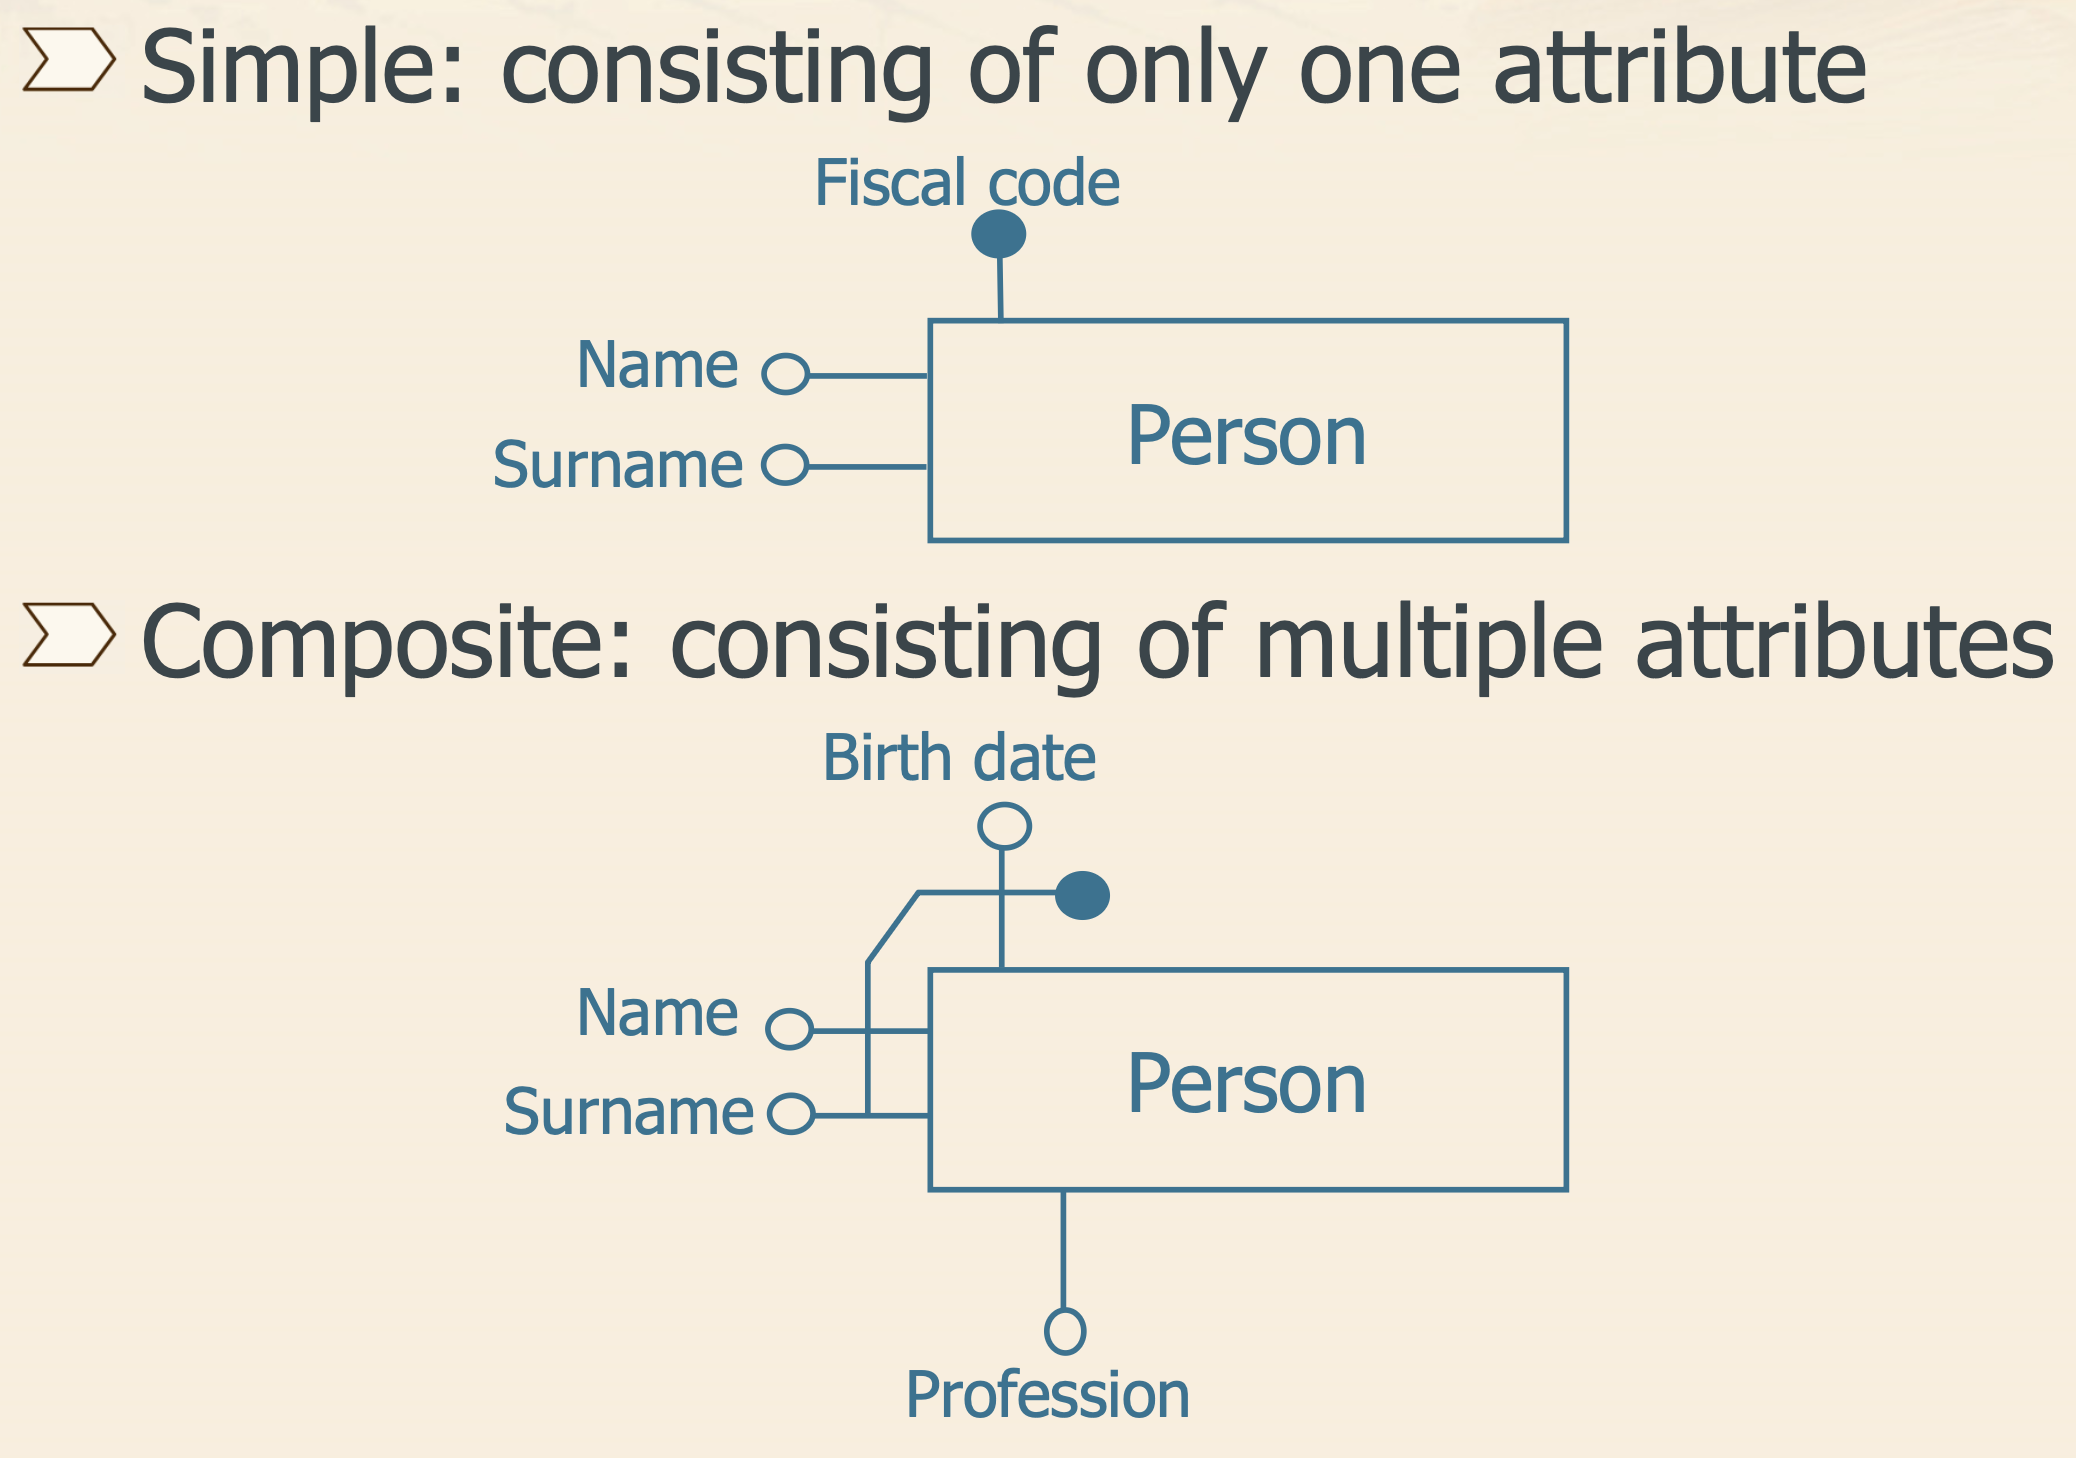
\includegraphics[width=0.7\textwidth]{immagini/er_attributi_semplici_composti.png} 
    \caption{Esempi di rappresentazione di attributi semplici (es. Codice Fiscale) e attributi composti (es. Data di Nascita) in un Diagramma ER.}
    \label{fig:er_attributi_semplici_composti}
\end{figure}

\subsubsection{Identificatori}
Gli identificatori permettono di distinguere univocamente le istanze di un'entità. Possono essere interni o esterni.
\begin{itemize}
    \item \textbf{Identificatore Interno}: Costituito da uno o più attributi dell'entità stessa (es. Codice Fiscale per Persona).
    \item \textbf{Identificatore Esterno}: Coinvolge attributi dell'entità e la partecipazione a relazioni con altre entità, necessarie per la sua identificazione. È tipico delle entità deboli.
\end{itemize}
\begin{figure}[h!]
    \centering
    \subcaptionbox{Identificatore Esterno per Entità Deboli (Studente, Immatricolazione, Università)\label{fig:er_entita_debole_enrollment}}{%
        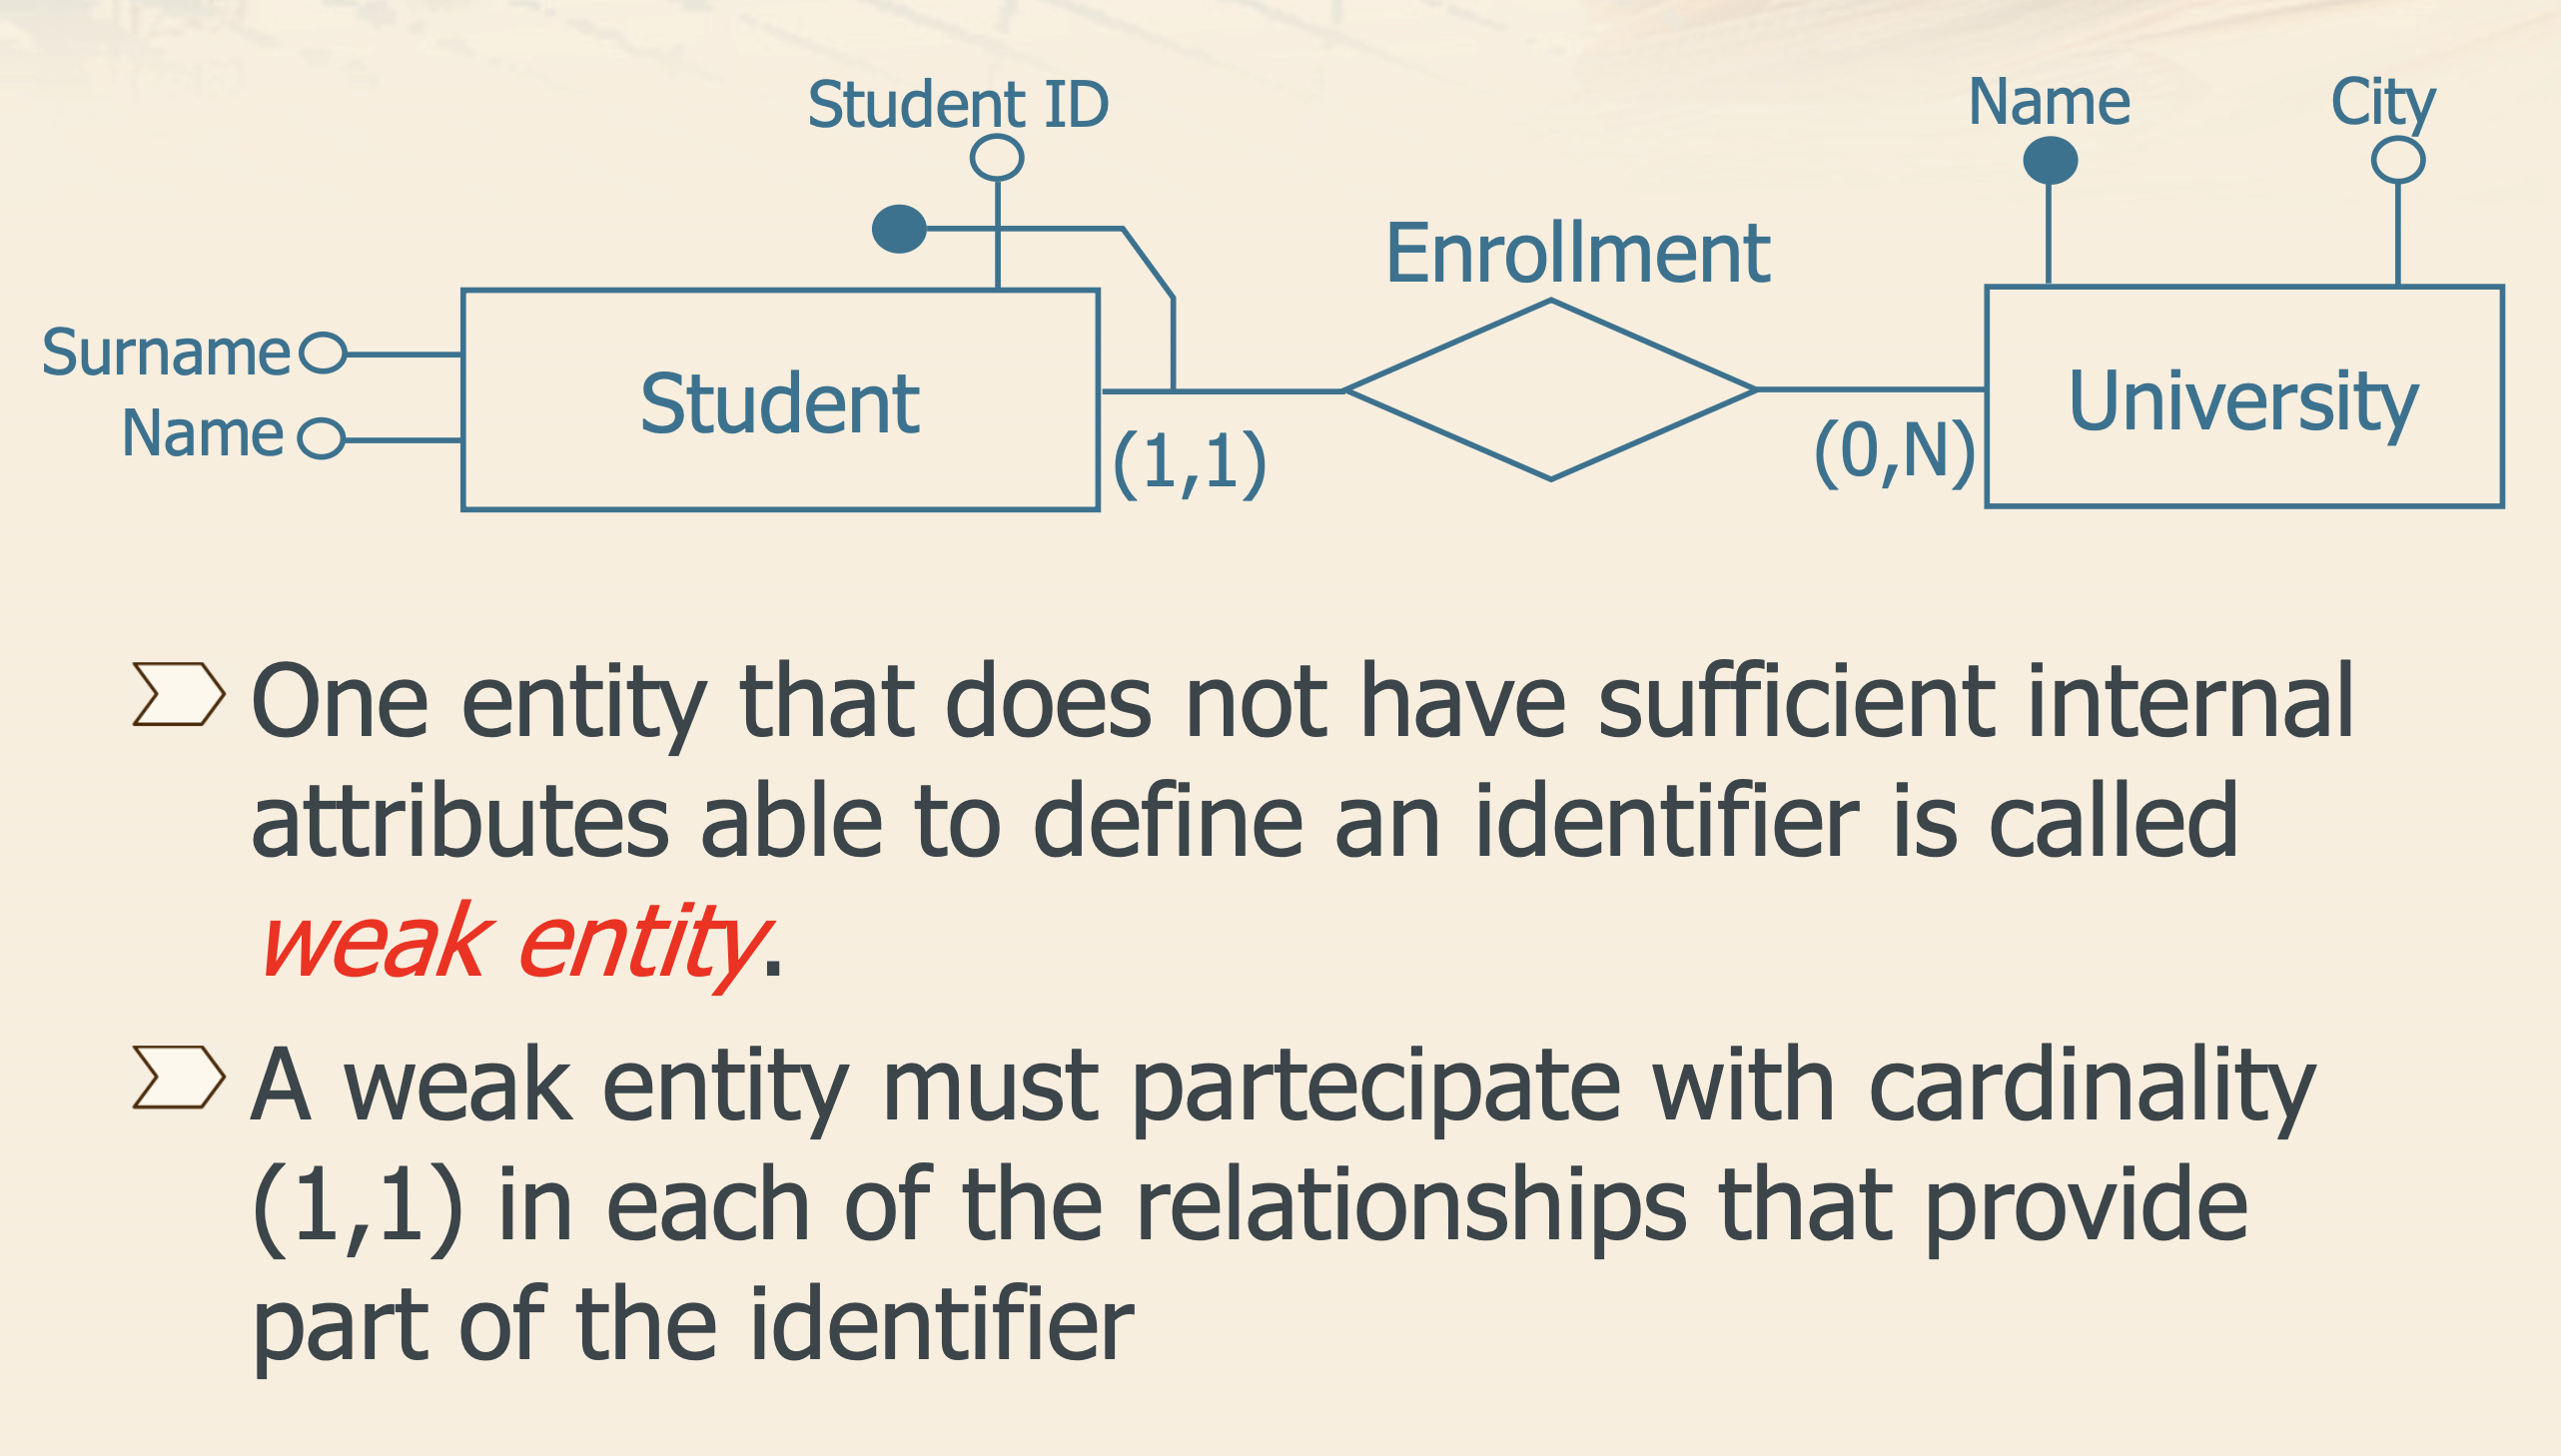
\includegraphics[width=0.48\textwidth]{immagini/er_entita_debole_enrollment.png}%
    }\quad
    \subcaptionbox{Identificatore Esterno Complesso (Stanza, Scaffale, Ripiano)\label{fig:er_identificatore_esterno_libreria}}{%
        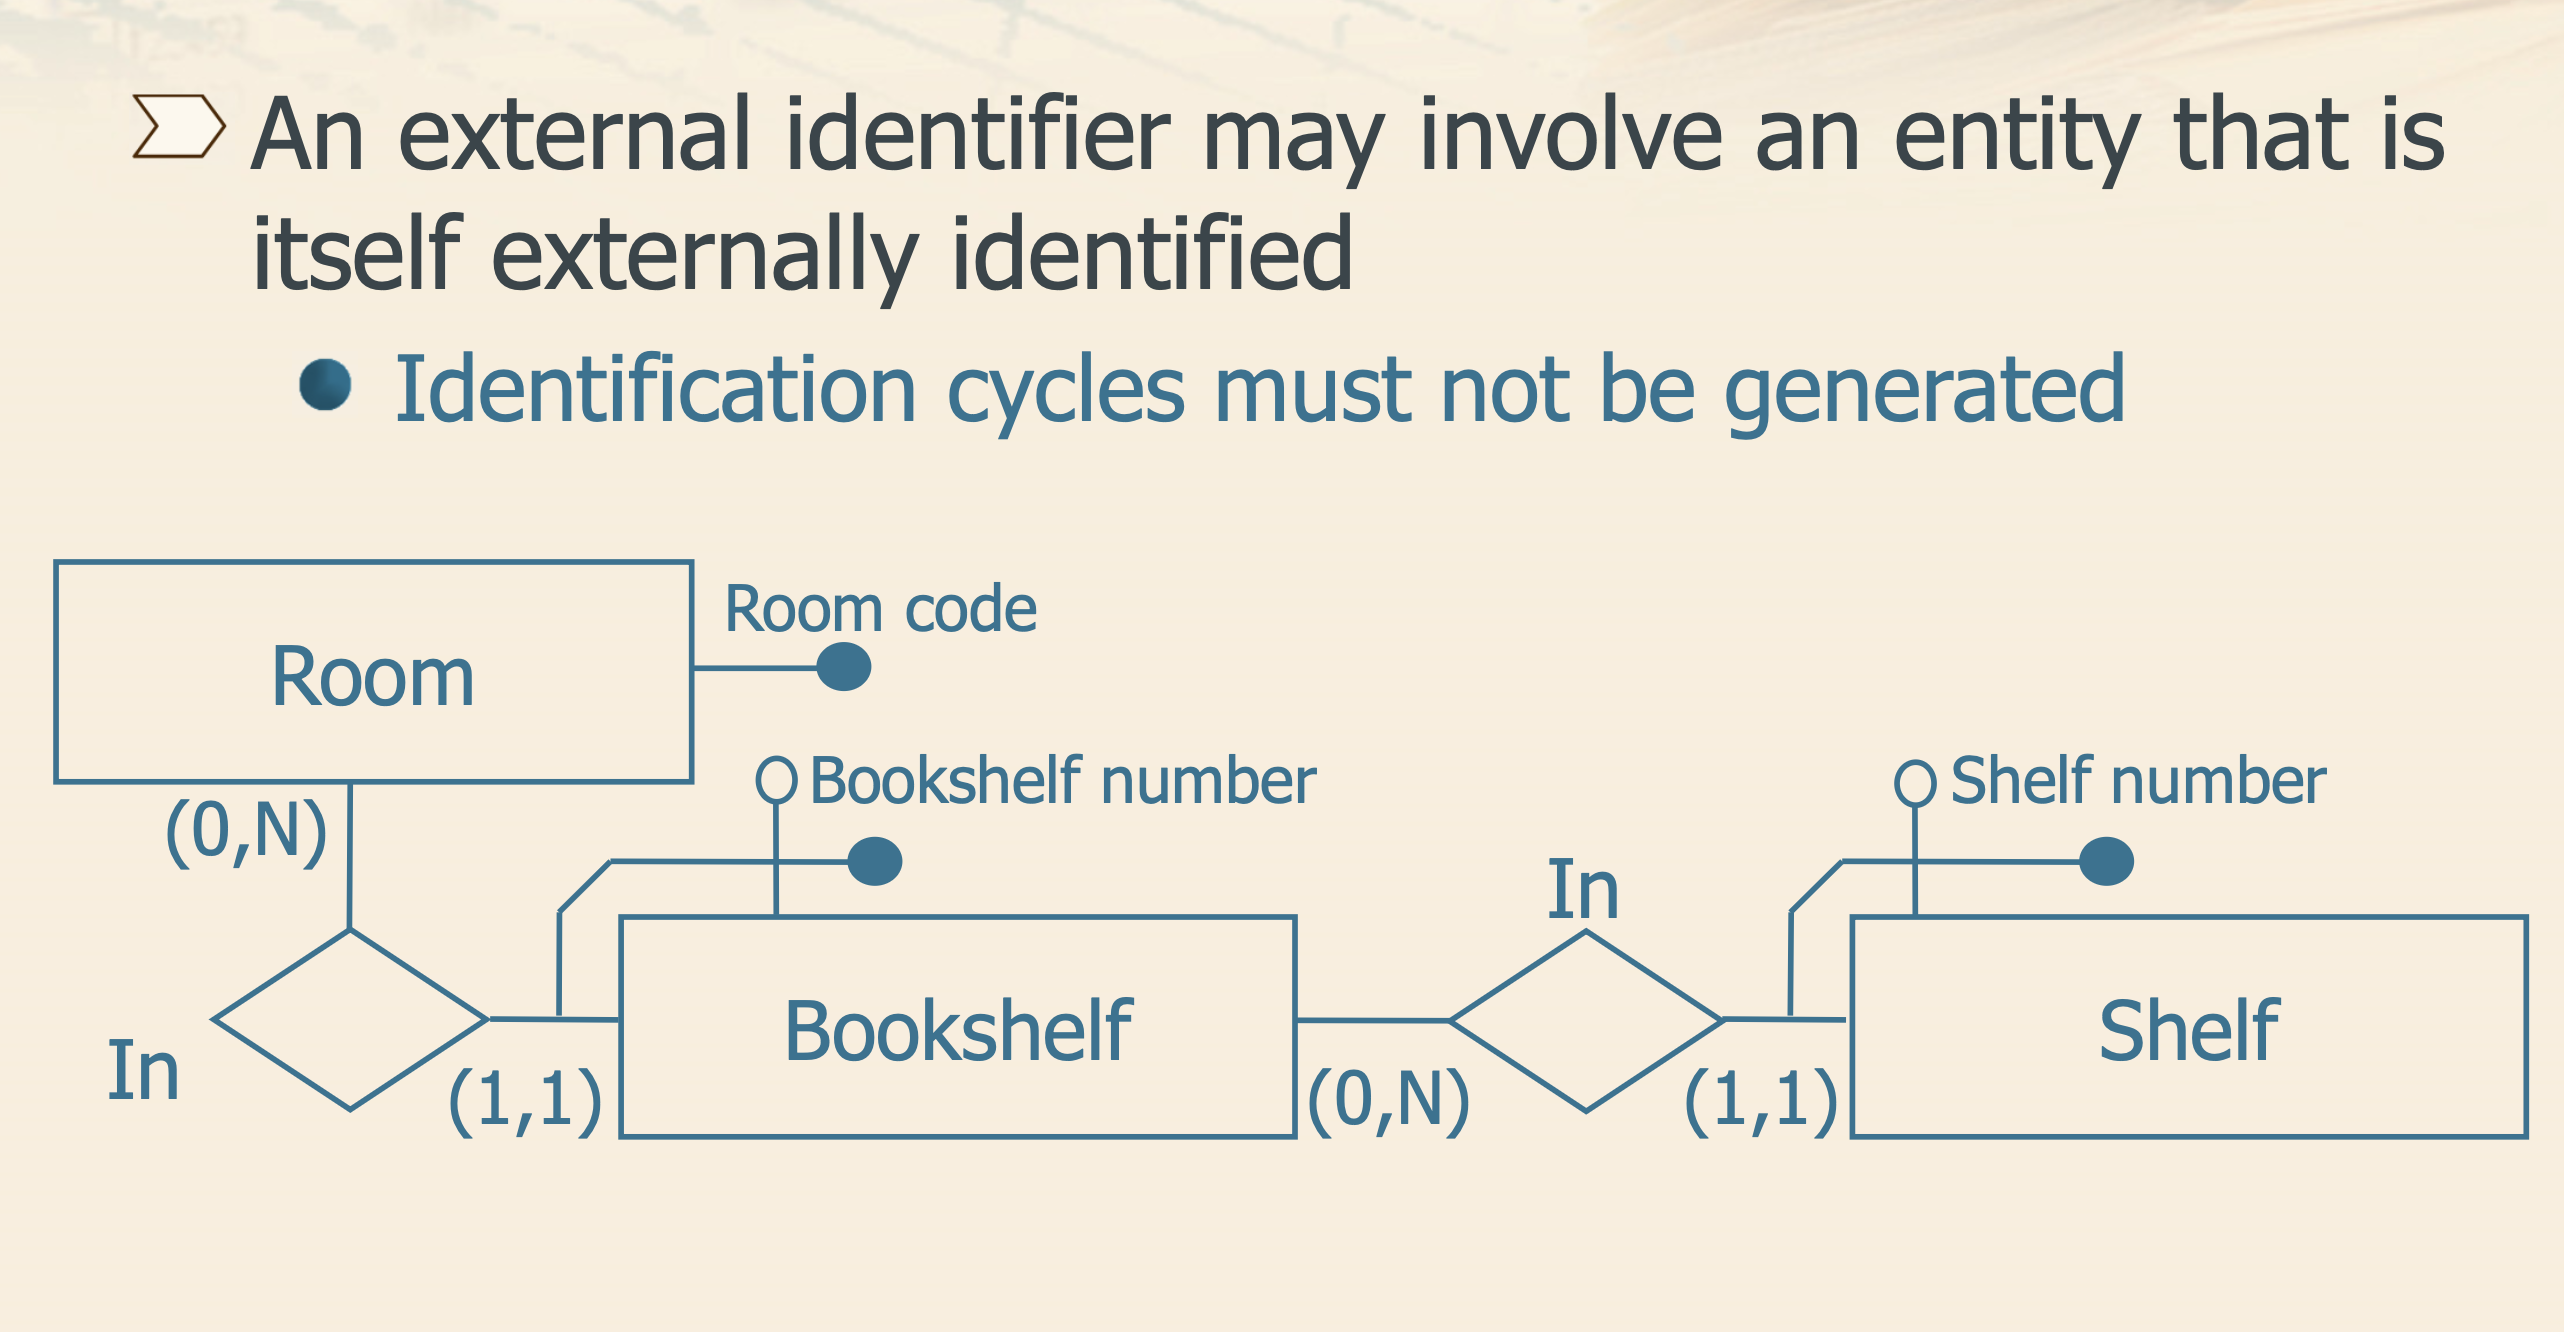
\includegraphics[width=0.48\textwidth]{immagini/er_identificatore_esterno_libreria.png}%
    }
    \caption{Esempi di utilizzo di identificatori esterni, inclusi scenari con entità deboli e concatenazione di identificazione.}
    \label{fig:er_identificatori_esterni}
\end{figure}

\subsection{Dettagli delle Relazioni e Cardinalità}
Le relazioni specificano le associazioni tra le entità, e le cardinalità definiscono il numero di istanze di un'entità che possono partecipare a una relazione.
\begin{itemize}
    \item \textbf{Cardinalità delle Relazioni}: Definisce il numero minimo e massimo di istanze di un'entità che possono essere associate a un'istanza dell'altra entità nella relazione.
    \begin{itemize}
        \item \textbf{Minima}: Indica se la partecipazione è obbligatoria (1) o opzionale (0).
        \item \textbf{Massima}: Indica il numero massimo di partecipazioni (1 o N).
        \item \textbf{Notazione (min, max)}: Es. $(0, N)$ per zero a molti, $(1, N)$ per uno a molti.
    \end{itemize}
    \item \textbf{Partecipazione (o Dipendenza)}:
    \begin{itemize}
        \item \textbf{Totale (o Obbligatoria)}: Ogni istanza dell'entità deve partecipare alla relazione (indicata graficamente da una doppia linea di connessione).
        \item \textbf{Parziale (o Opzionale)}: Un'istanza dell'entità può partecipare o meno alla relazione (indicata graficamente da una singola linea).
    \end{itemize}
\end{itemize}

\subsection{Generalizzazione nel Modello ER}
La \textbf{Generalizzazione} è un costrutto del modello ER che permette di rappresentare una relazione "è un tipo di" (is-a) tra un'entità genitore (generale) e una o più entità figlie (specializzate).
\begin{itemize}
    \item Ogni istanza di un'entità figlia è anche un'istanza dell'entità genitore.
    \item Le proprietà (attributi, identificatori, relazioni) dell'entità genitore sono ereditate da tutte le entità figlie.
\end{itemize}
\begin{figure}[h!]
    \centering
    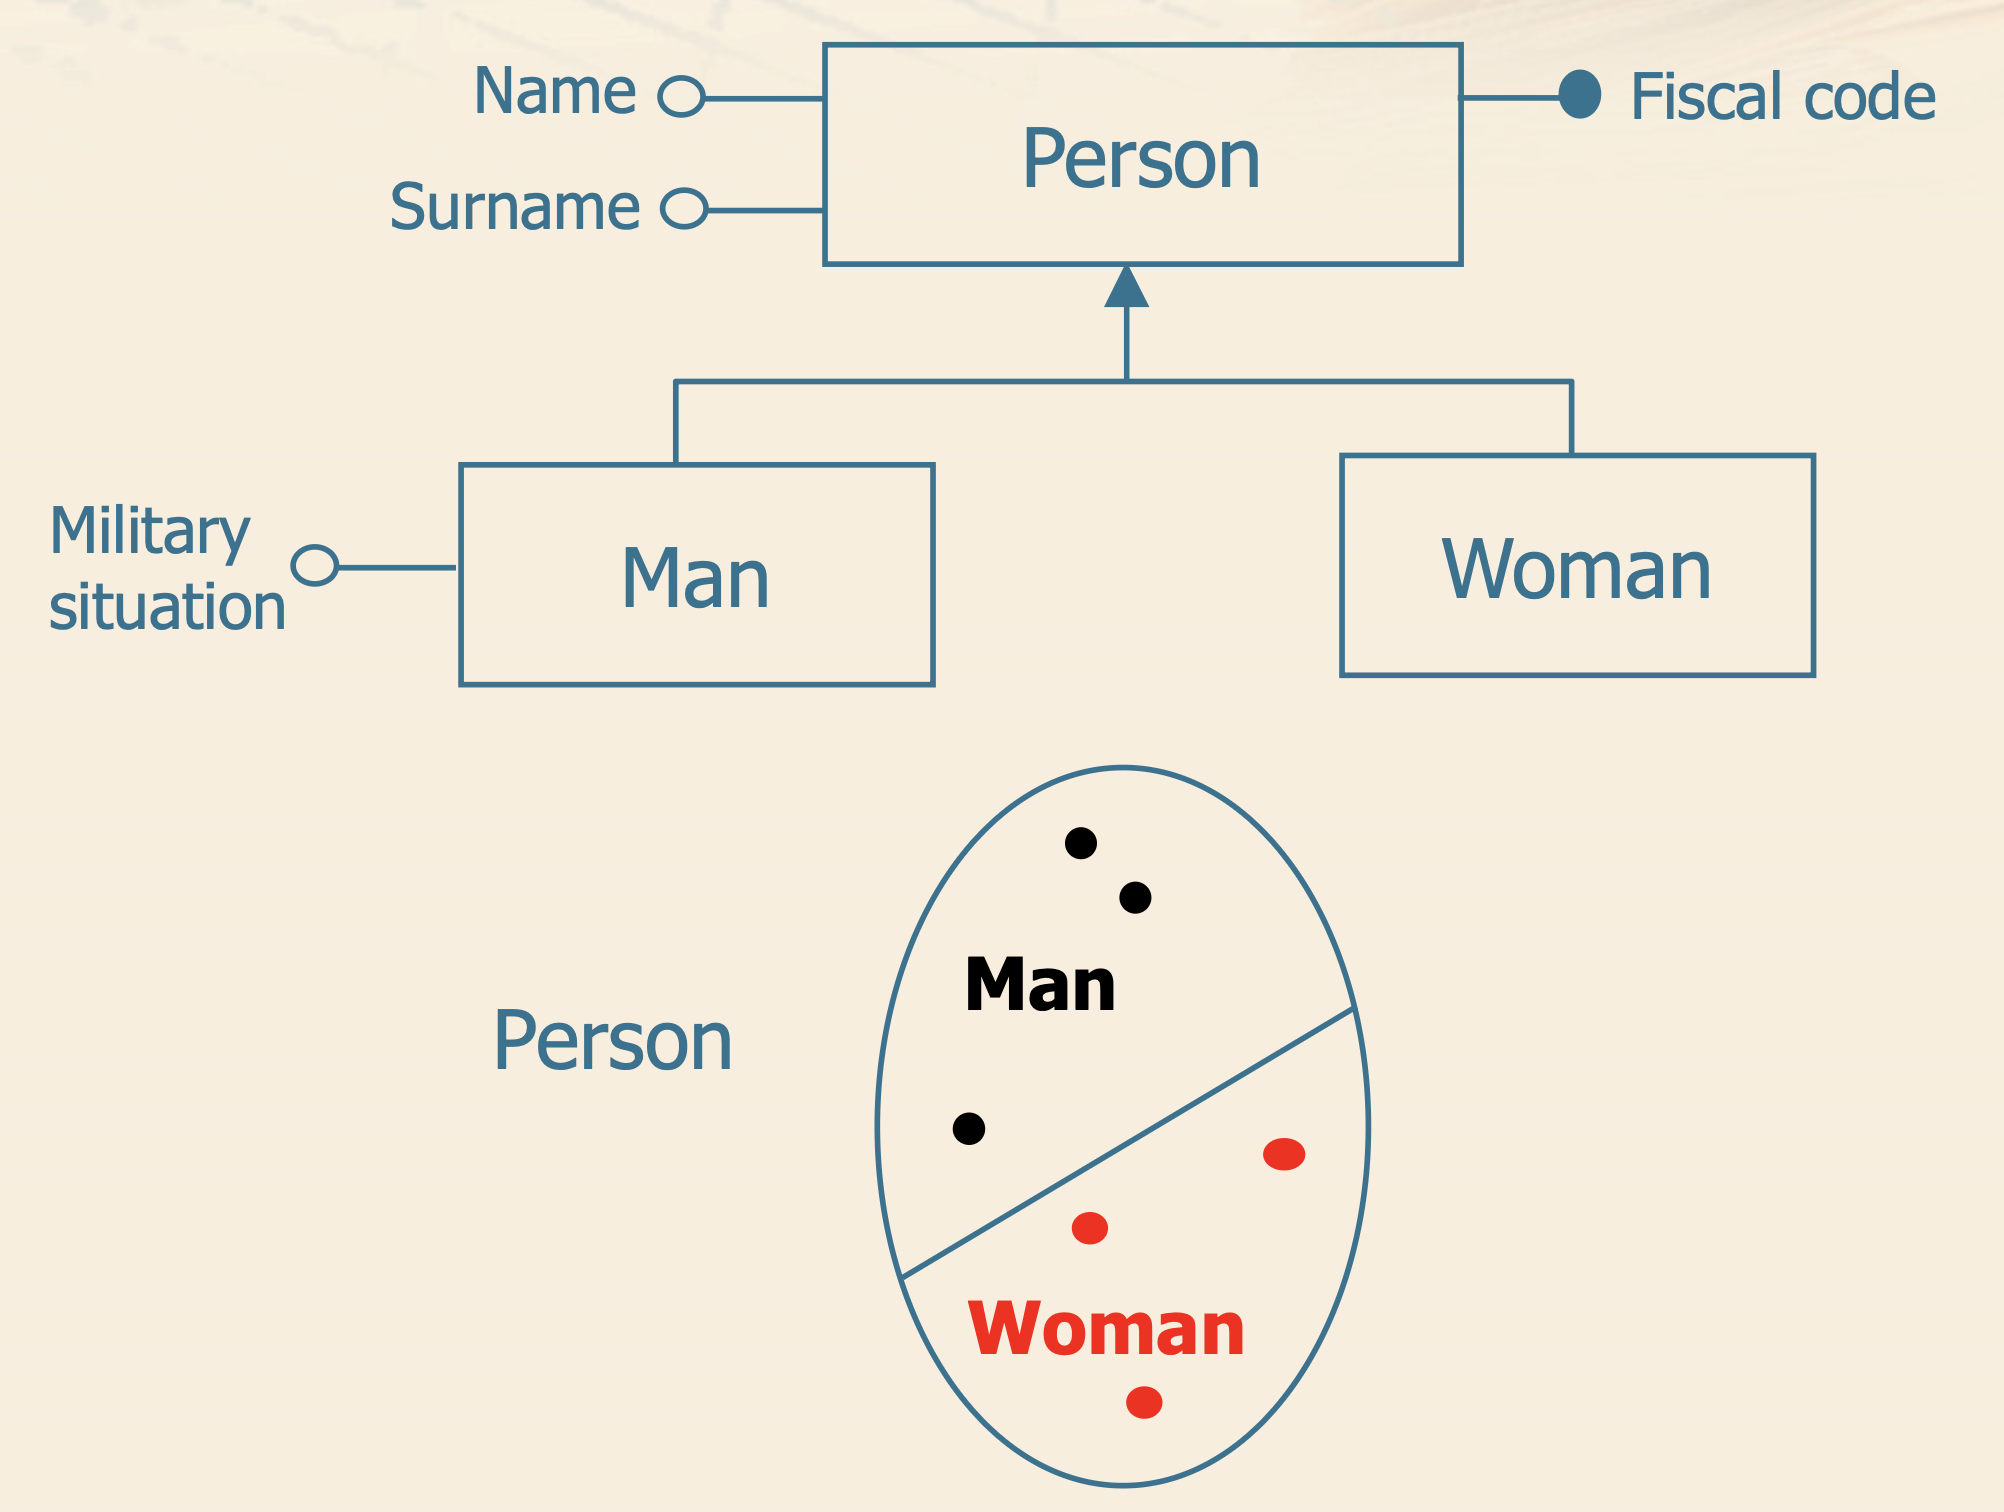
\includegraphics[width=0.7\textwidth]{immagini/er_generalizzazione_person_gender.png} % Immagine dal tuo screenshot 16.08.24.jpg
    \caption{Esempio di Generalizzazione nel Diagramma ER: l'entità Persona si generalizza nelle entità Uomo e Donna, mostrando la distinzione e l'ereditarietà delle proprietà.}
    \label{fig:er_generalizzazione_person_gender}
\end{figure}

\subsection{Esempi Complessi di Schemi ER}
Per consolidare la comprensione del Modello ER, è utile analizzare esempi complessi che integrano vari concetti come entità, attributi, relazioni con cardinalità diverse, identificatori, generalizzazioni e entità deboli. Questi schemi rappresentano contesti reali e mostrano come i costrutti ER vengono applicati per modellare domini complessi.

\begin{figure}[h!]
    \centering
    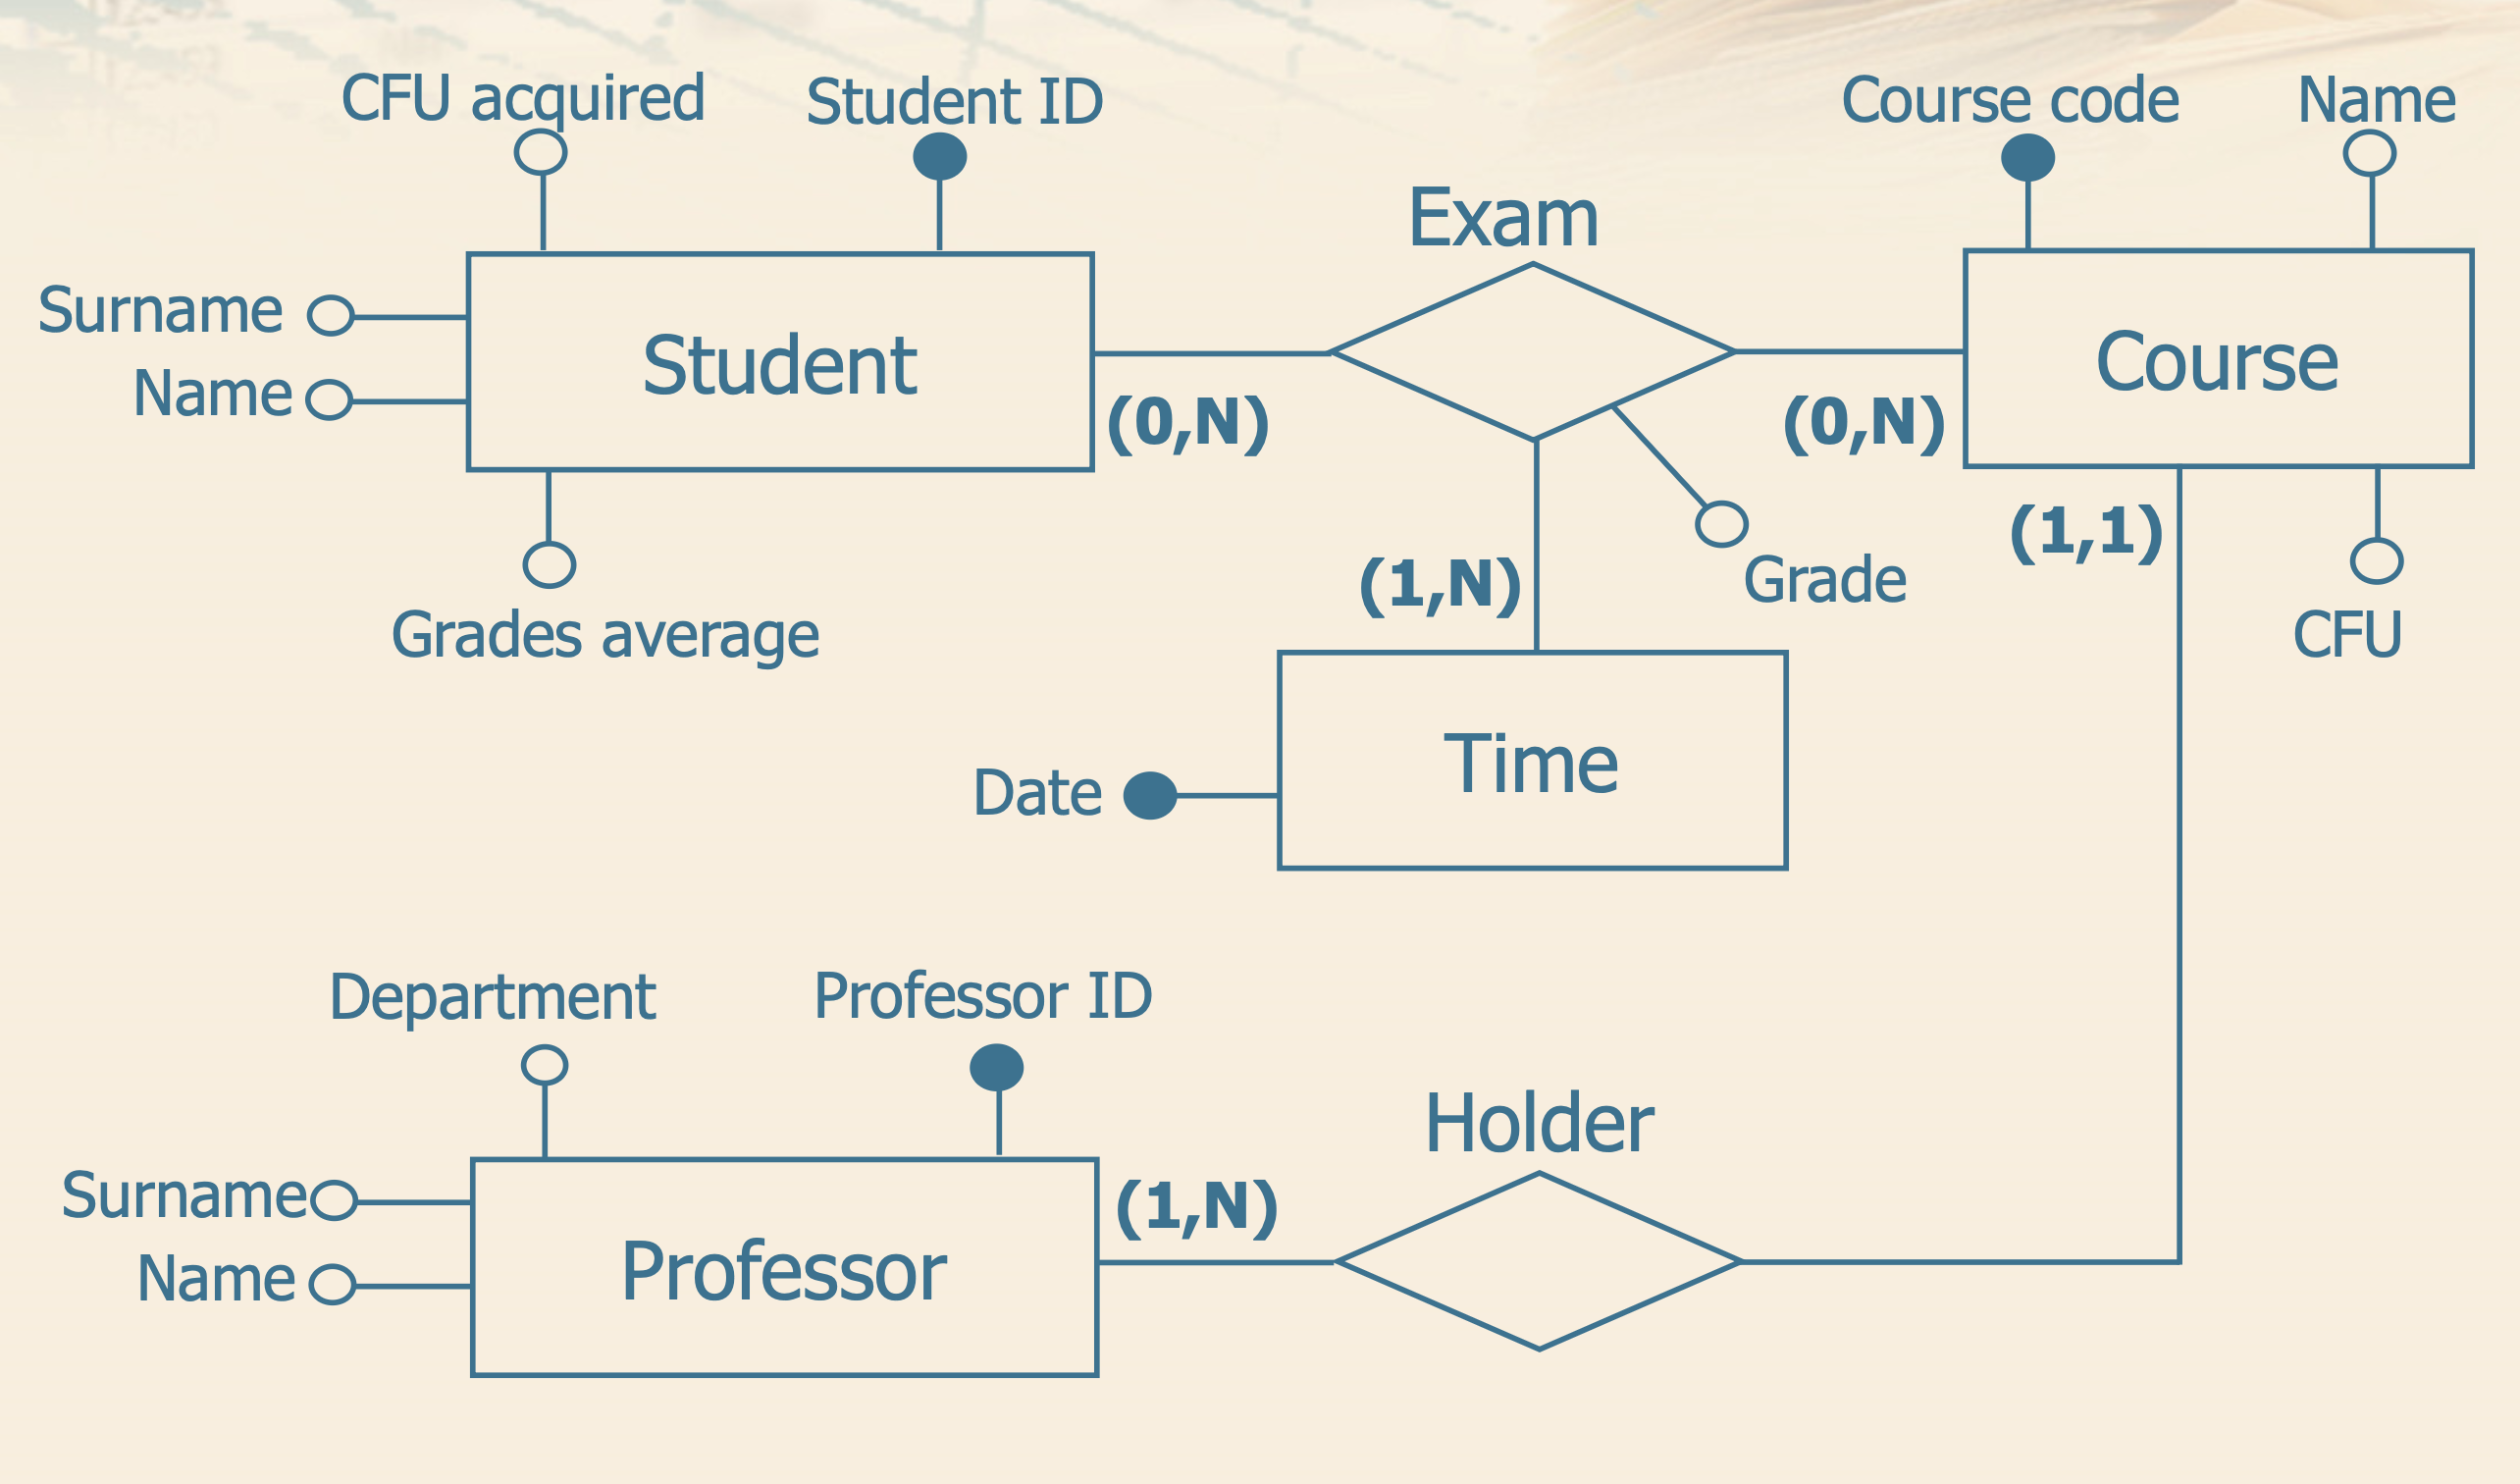
\includegraphics[width=0.9\textwidth]{immagini/er_schema_student_course_exam.png} % Immagine dal tuo screenshot 16.09.49.jpg
    \caption{Diagramma ER che modella le relazioni tra Studenti, Corsi ed Esami, inclusi attributi e cardinalità.}
    \label{fig:er_schema_student_course_exam}
\end{figure}

\subsection{Esempi Complessi di Schemi ER}
Per consolidare la comprensione del Modello ER, è utile analizzare esempi complessi che integrano vari concetti come entità, attributi, relazioni con cardinalità diverse, identificatori, generalizzazioni e entità deboli. Questi schemi rappresentano contesti reali e mostrano come i costrutti ER vengono applicati per modellare domini complessi.

\begin{figure}[h!]
    \centering
    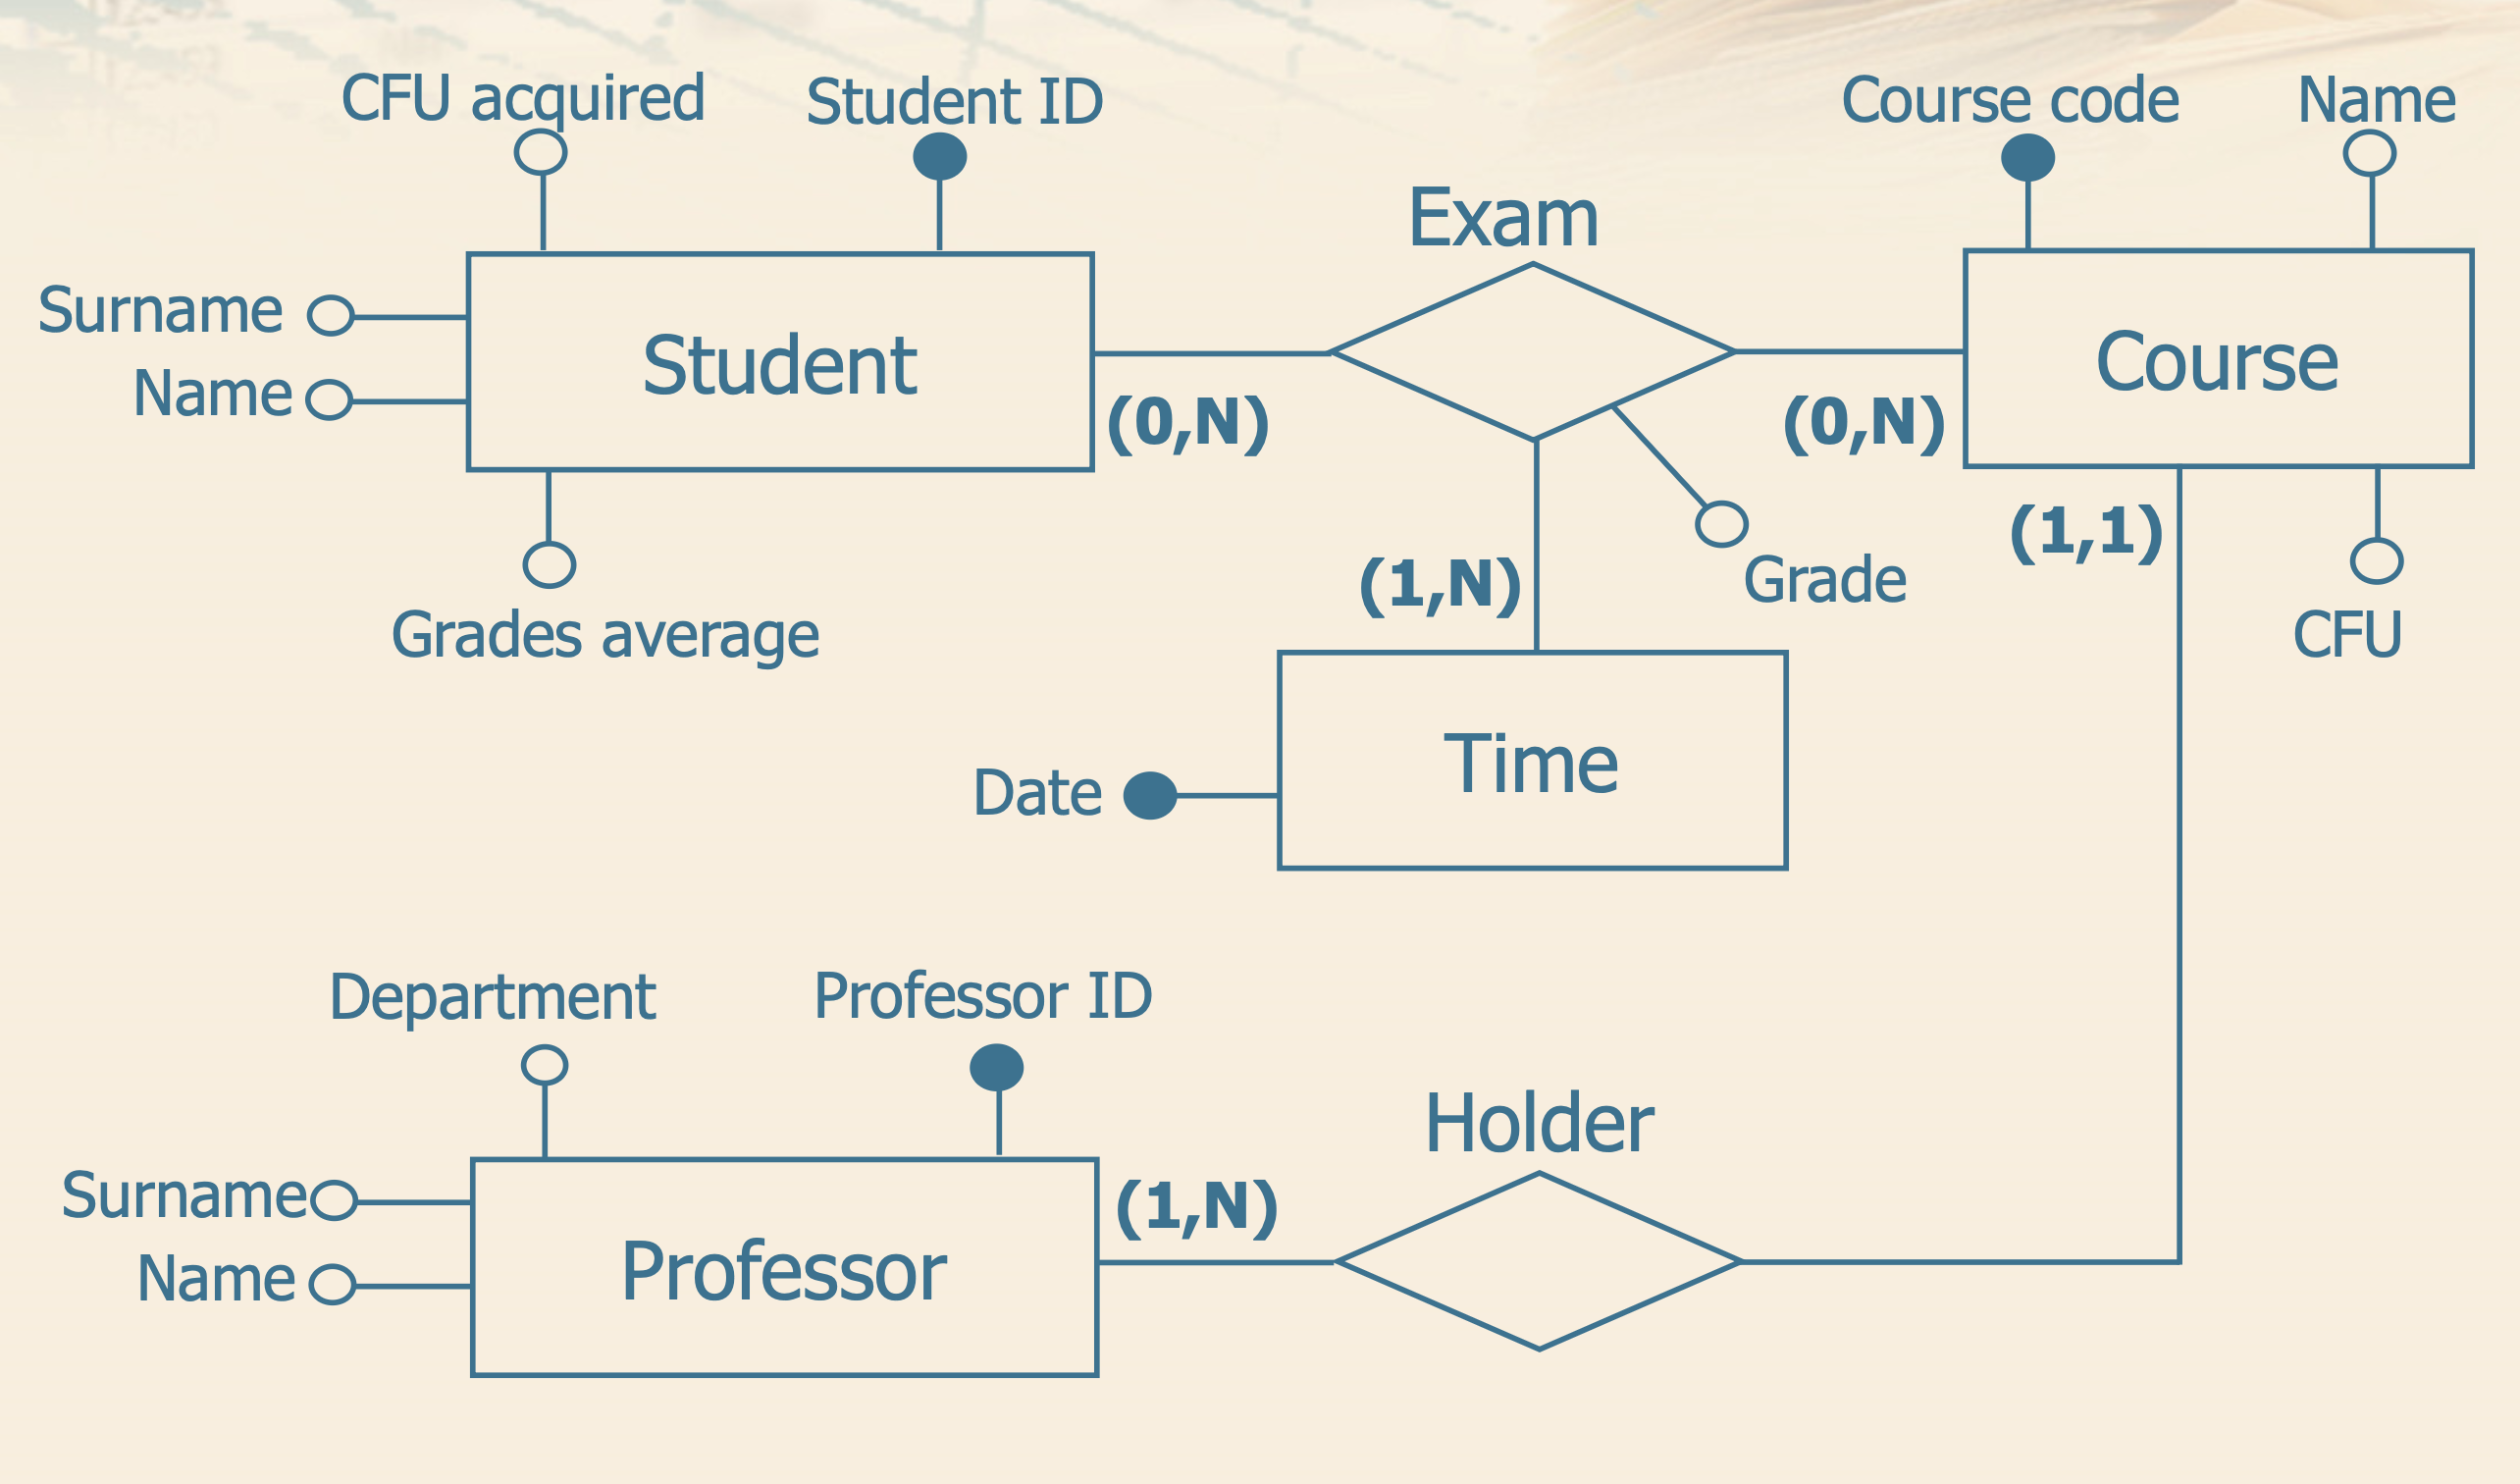
\includegraphics[width=0.9\textwidth]{immagini/er_schema_student_course_exam.png} % Immagine dal tuo screenshot 16.09.49.jpg
    \caption{Diagramma ER che modella le relazioni tra Studenti, Corsi ed Esami, inclusi attributi e cardinalità.}
    \label{fig:er_schema_student_course_exam}
\end{figure}

\subsubsection{Esercizio 2: Sistema Cinema/Film}
\textbf{Descrizione}: Si consideri uno schema Entità-Relazione che rappresenta un sistema per la gestione di film, artisti, cinema e città. Il diagramma include entità come Film, Artista, Cinema e Città, con relazioni che specificano la regia, l'interpretazione e la proiezione dei film nei cinema locali.
\begin{figure}[h!]
    \centering
    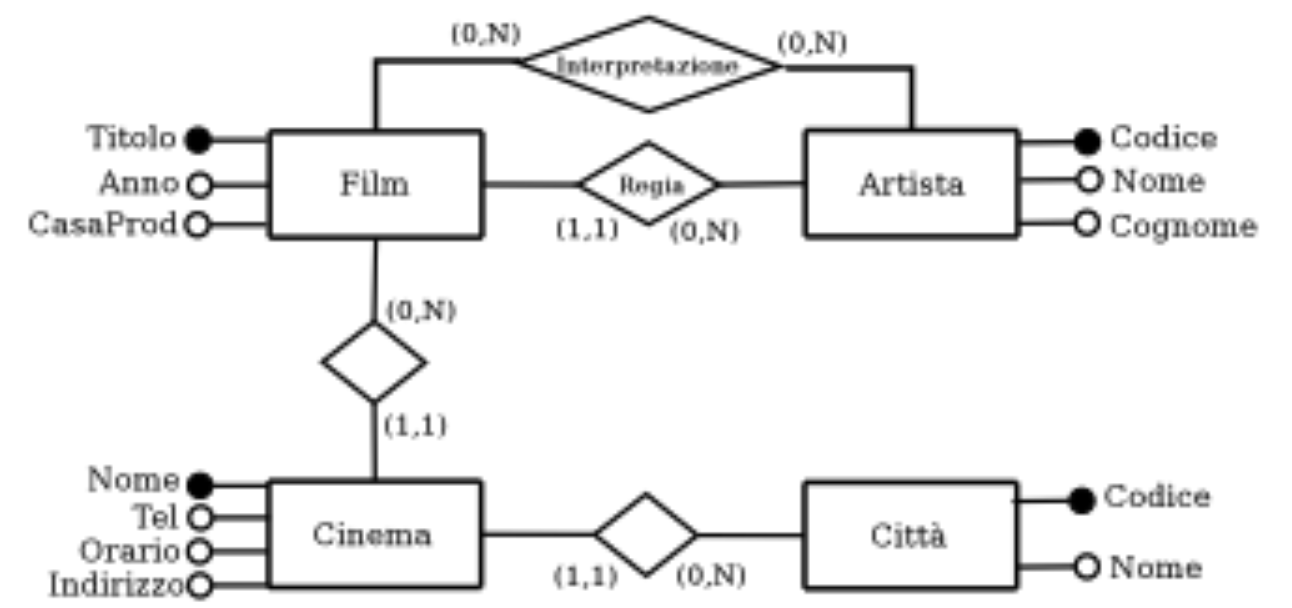
\includegraphics[width=0.9\textwidth]{immagini/er_esercizio_2_cinema_film.png} % Immagine da eserciziER.pdf, Pagina 1, Figura 1
    \caption{Schema ER per l'esercizio 2: Sistema Cinema/Film.}
    \label{fig:er_esercizio_2_cinema_film}
\end{figure}

\textbf{Schema Relazionale corrispondente}:
\begin{lstlisting}[language=SQL]
ARTISTI (Codice, Nome, Cognome)
FILM (Titolo, Anno, CasaProduttrice, RegistaArtista) -- RegistaArtista FK a ARTISTI
INTERPRETAZIONI (FilmTitolo, FilmAnno, ArtistaCodice) -- FK a FILM, FK a ARTISTI
CITTA (Codice, Nome)
CINEMA (Nome, Tel, Orario, Indirizzo, CittaCodice) -- CittaCodice FK a CITTA
PROIEZIONI (FilmTitolo, FilmAnno, CinemaNome, OrarioCinema) -- FK a FILM, FK a CINEMA
\end{lstlisting}

\subsubsection{Esercizio 7: Sistema Campionato di Calcio}
\textbf{Descrizione}: Modellare un sistema per la gestione di un campionato di calcio. Il sistema deve rappresentare squadre, giocatori (con i loro ruoli e dati personali), arbitri, giornate e partite, inclusi i risultati e le specificità come partite in campo neutro o rinviate.
\begin{figure}[h!]
    \centering
    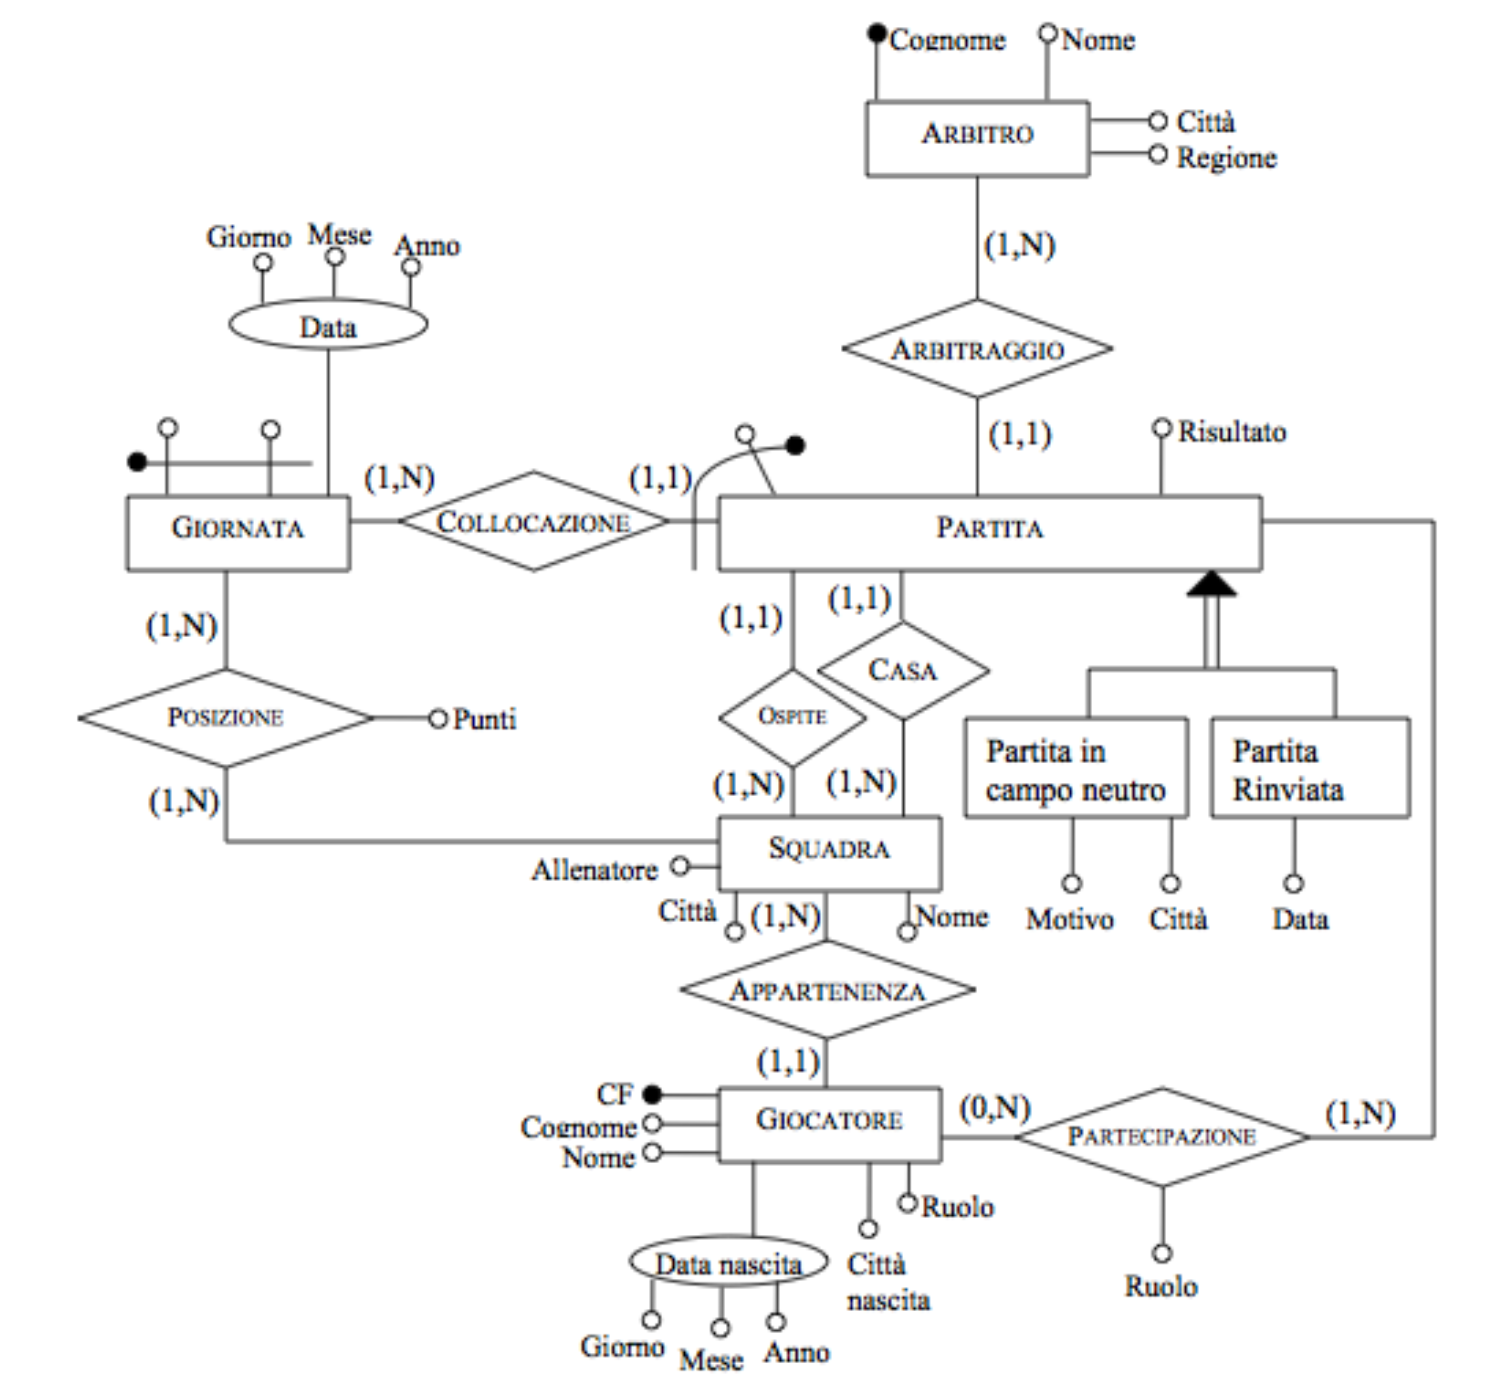
\includegraphics[width=0.9\textwidth]{immagini/er_esercizio_7_campionato_calcio.png} % Immagine da eserciziER.pdf, Pagina 3, Figura 6
    \caption{Schema ER per l'esercizio 7: Sistema Campionato di Calcio.}
    \label{fig:er_esercizio_7_campionato_calcio}
\end{figure}

\textbf{Schema Relazionale corrispondente}:
\begin{lstlisting}[language=SQL]
ARBITRO (Cognome, Nome, Citta, Regione) -- Chiave primaria (Cognome, Nome) o ID_Arbitro generato
GIORNATA (Numero, Serie, Giorno, Mese, Anno) -- Chiave primaria (Numero, Serie)
SQUADRA (Nome, Citta, Allenatore) -- Chiave primaria (Nome)
GIOCATORE (CodiceFiscale, Cognome, Nome, Ruolo, CittaDiNascita) -- Chiave primaria (CodiceFiscale)
PARTITA (NumeroPartita, GiornoGiornata, MeseGiornata, AnnoGiornata, Risultato, ArbitroCognome, ArbitroNome, CasaSquadra, OspiteSquadra) -- Chiave primaria (NumeroPartita), FK a GIORNATA, FK a ARBITRO, FK a SQUADRA (due volte)
PARTITA_IN_CAMPO_NEUTRO (PartitaNumero, PartitaGiorno, PartitaMese, PartitaAnno, Motivo, CittaCampoNeutro) -- FK a PARTITA
PARTITA_RINVIATA (PartitaNumero, PartitaGiorno, PartitaMese, PartitaAnno, DataRinvio) -- FK a PARTITA
POSIZIONE (SquadraNome, GiornoGiornata, MeseGiornata, AnnoGiornata, Punteggio) -- Chiave primaria (SquadraNome, GiornoGiornata, MeseGiornata, AnnoGiornata), FK a SQUADRA, FK a GIORNATA
APPARTENENZA (GiocatoreCodiceFiscale, SquadraNome, DataInizio, RuoloPrincipale, DataFine) -- Chiave primaria (GiocatoreCodiceFiscale, SquadraNome, DataInizio), FK a GIOCATORE, FK a SQUADRA
\end{lstlisting}

\subsubsection{Esercizio 11: Sistema Gare Ciclistiche}
\textbf{Descrizione}: Un sistema per la gestione di gare ciclistiche, includendo informazioni su ciclisti, squadre, località, competizioni, edizioni e tappe, con dettagli sulle classifiche e gli orari.
\begin{figure}[h!]
    \centering
    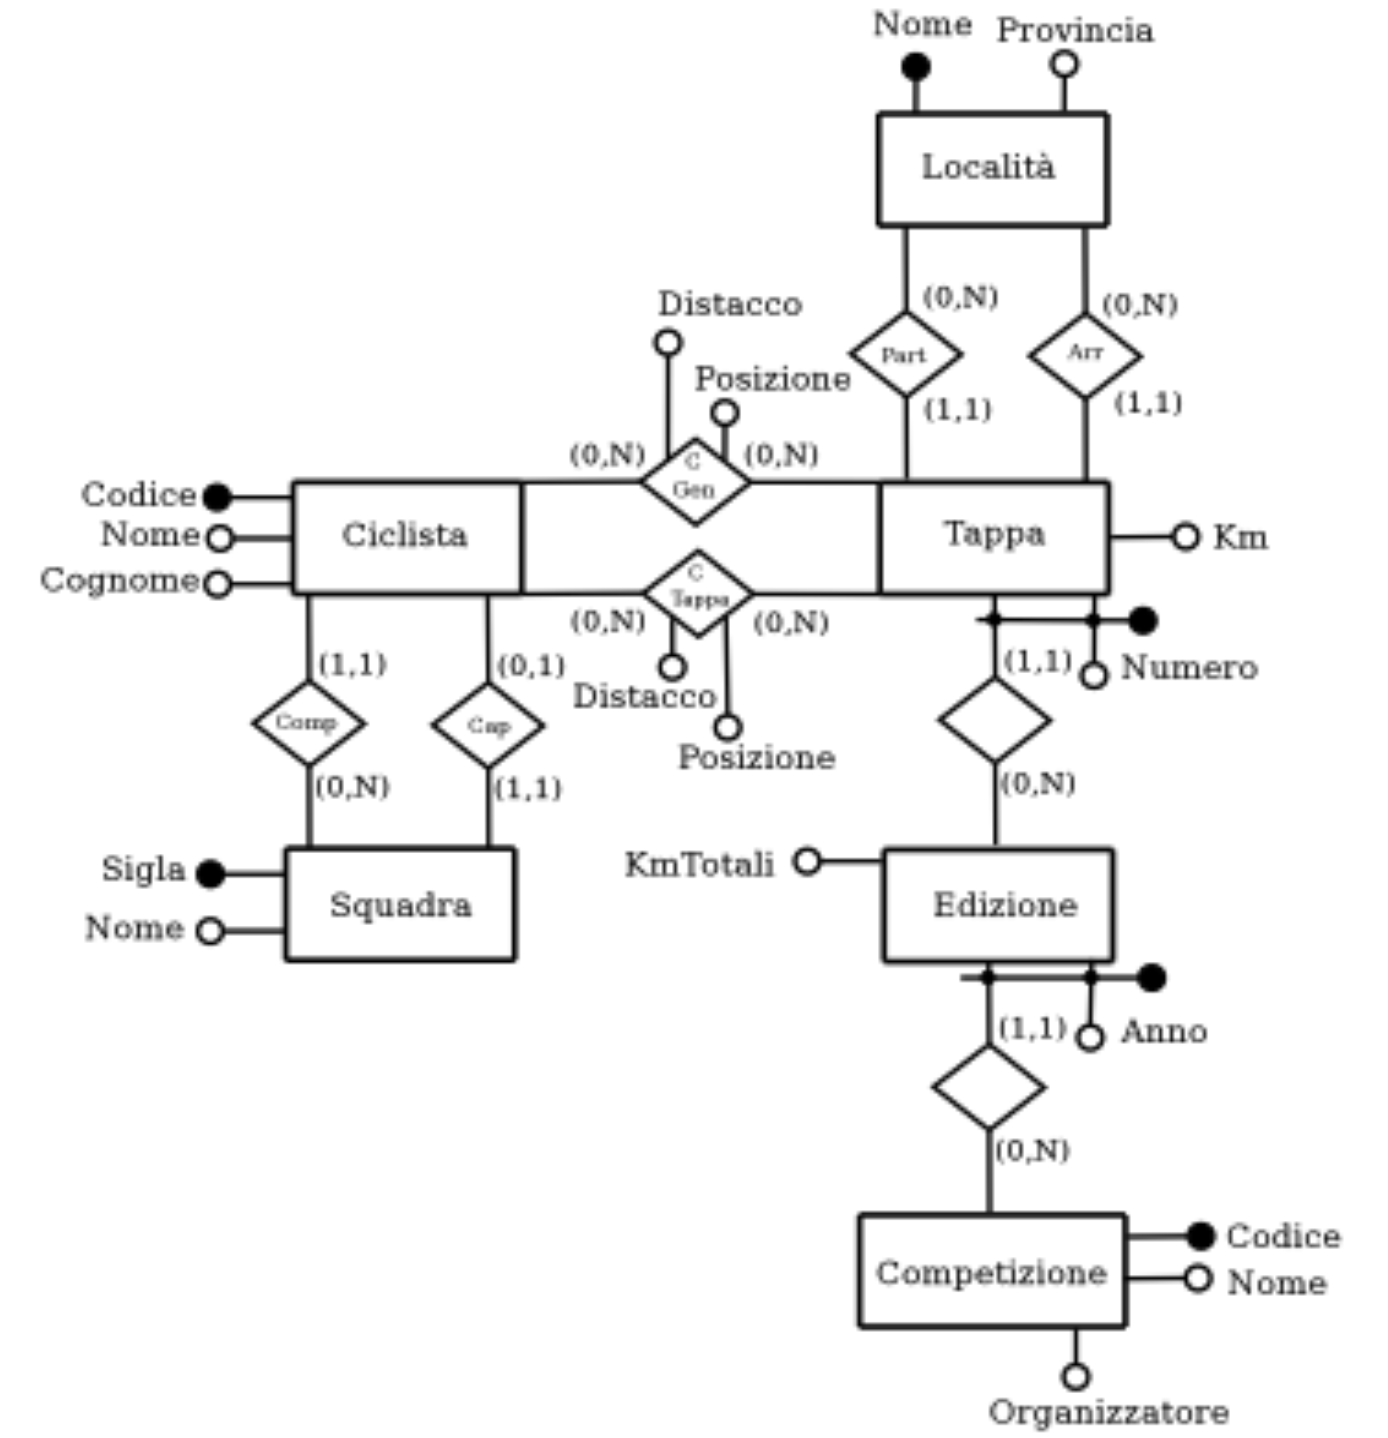
\includegraphics[width=0.9\textwidth]{immagini/er_esercizio_11_ciclisti_tappa.png} % Immagine da eserciziER.pdf, Pagina 5, Figura 10
    \caption{Schema ER per l'esercizio 11: Sistema Gare Ciclistiche.}
    \label{fig:er_esercizio_11_ciclisti_tappa}
\end{figure}

\textbf{Schema Relazionale corrispondente}:
\begin{lstlisting}[language=SQL]
SQUADRE (Sigla, Nome, CapitanoCodice) -- CapitanoCodice FK a CICLISTI
CICLISTI (Codice, Cognome, Nome, SquadraSigla) -- SquadraSigla FK a SQUADRE
LOCALITA (Nome, Provincia) -- Chiave primaria (Nome, Provincia)
COMPETIZIONI (Codice, Nome, Organizzatore) -- Chiave primaria (Codice)
EDIZIONI (AnnoEdizione, CompetizioneCodice, KmTotali) -- Chiave primaria (AnnoEdizione, CompetizioneCodice), FK a COMPETIZIONI
TAPPE (NumeroTappa, AnnoEdizione, CompetizioneCodice, LocPartenzaNome, LocPartenzaProvincia, LocArrivoNome, LocArrivoProvincia) -- Chiave primaria (NumeroTappa, AnnoEdizione, CompetizioneCodice), FK a EDIZIONI, FK a LOCALITA (due volte)
CLASSIFICATAPPA (NumeroTappa, AnnoEdizione, CompetizioneCodice, CiclistaCodice, Posizione, Distacco) -- FK a TAPPE, FK a CICLISTI
CLASSIFICAGENERALE (NumeroTappa, AnnoEdizione, CompetizioneCodice, CiclistaCodice, Posizione, Distacco) -- FK a TAPPE, FK a CICLISTI
\end{lstlisting}

\section{Progettazione Logica: Normalizzazione e Forme Normali}
La \textbf{normalizzazione} è un processo sistematico di organizzazione dei dati in un database relazionale. Il suo scopo è ridurre la ridondanza dei dati, eliminare le anomalie di aggiornamento (inserimento, cancellazione, modifica) e migliorare l'integrità e la coerenza dei dati. La normalizzazione si basa su una serie di regole chiamate "forme normali".

\subsection{Obiettivi della Normalizzazione}
\begin{itemize}
    \item \textbf{Riduzione della Ridondanza}: Evitare la duplicazione inutile dei dati, che spreca spazio e può portare a incongruenze.
    \item \textbf{Miglioramento dell'Integrità dei Dati}: Assicurare che i dati siano accurati e consistenti.
    \item \textbf{Prevenzione delle Anomalie}:
    \begin{itemize}
        \item \textbf{Anomalia di Inserimento}: Impossibilità di inserire un'informazione a meno che non si inseriscano anche altre informazioni non correlate.
        \item \textbf{Anomalia di Cancellazione}: La cancellazione di un dato comporta la perdita accidentale di altre informazioni non desiderate.
        \item \textbf{Anomalia di Aggiornamento}: La modifica di un dato ripetuto richiede l'aggiornamento di più occorrenze, con rischio di inconsistenza se non tutte vengono aggiornate.
    \end{itemize}
    \item \textbf{Flessibilità e Manutenibilità}: Rendere il database più facile da modificare ed estendere.
\end{itemize}

\subsection{Principali Forme Normali}
Le forme normali sono una serie di regole progressive; per essere in una forma normale N, una relazione deve soddisfare i requisiti della forma normale N-1. Le più comuni e rilevanti per la maggior parte delle applicazioni sono la Prima, Seconda e Terza Forma Normale.

\subsubsection{Prima Forma Normale (1NF)}
Una relazione è in 1NF se e solo se:
\begin{itemize}
    \item Tutti gli attributi sono \textbf{atomici} (indivisibili). Non ci sono attributi con valori multipli o attributi composti che non sono stati scomposti.
    \item Ogni record (riga) nella relazione è \textbf{unico}. Questo implica che deve esistere una chiave primaria.
\end{itemize}
\textbf{Esempio di Violazione}: Una colonna "NumeriDiTelefono" che contiene più numeri per un'unica riga.

\subsubsection{Seconda Forma Normale (2NF)}
Una relazione è in 2NF se e solo se:
\begin{itemize}
    \item È in \textbf{1NF}.
    \item Tutti gli attributi non-chiave dipendono \textbf{completamente} dalla chiave primaria. Non ci sono dipendenze parziali, il che significa che nessun attributo non-chiave dipende solo da una parte di una chiave primaria composta.
\end{itemize}
\textbf{Esempio di Violazione}: In una tabella `(IDCorso, IDStudente, NomeCorso, Voto)`, se `(IDCorso, IDStudente)` è la chiave primaria, e `NomeCorso` dipende solo da `IDCorso` (e non da `IDStudente`), allora `NomeCorso` è parzialmente dipendente e viola la 2NF.

\subsubsection{Terza Forma Normale (3NF)}
Una relazione è in 3NF se e solo se:
\begin{itemize}
    \item È in \textbf{2NF}.
    \item Non contiene \textbf{dipendenze transitive}. Ovvero, nessun attributo non-chiave dipende da un altro attributo non-chiave (anziché dipendere direttamente dalla chiave primaria).
\end{itemize}
\textbf{Esempio di Violazione}: In una tabella `(IDImpiegato, NomeImpiegato, Dipartimento, CapoDipartimento)`, se `IDImpiegato` è la chiave primaria e `CapoDipartimento` dipende da `Dipartimento` (che a sua volta dipende da `IDImpiegato`), si ha una dipendenza transitiva.

\subsection{Linguaggio SQL}
Il \textbf{Structured Query Language (SQL)} è il linguaggio standard per la gestione dei sistemi di gestione di database relazionali (RDBMS). Permette di definire, manipolare e controllare i dati.

\subsubsection{Categorie di Comandi SQL}
\begin{itemize}
    \item \textbf{Data Definition Language (DDL)}: Utilizzato per definire e modificare la struttura del database.
    \begin{itemize}
        \item \textbf{CREATE}: Crea database, tabelle, viste, indici, ecc. (es. `CREATE TABLE Studenti (...)`).
        \item \textbf{ALTER}: Modifica la struttura di oggetti esistenti (es. `ALTER TABLE Studenti ADD COLUMN Età INT`).
        \item \textbf{DROP}: Cancella oggetti dal database (es. `DROP TABLE Studenti`).
    \end{itemize}
    \item \textbf{Data Manipulation Language (DML)}: Utilizzato per manipolare i dati all'interno delle tabelle.
    \begin{itemize}
        \item \textbf{SELECT}: Recupera dati da una o più tabelle. È la query più usata.
        \item \textbf{INSERT}: Aggiunge nuove righe a una tabella.
        \item \textbf{UPDATE}: Modifica righe esistenti in una tabella.
        \item \textbf{DELETE}: Rimuove righe da una tabella.
    \end{itemize}
    \item \textbf{Data Control Language (DCL)}: Utilizzato per gestire i permessi di accesso ai dati.
    \begin{itemize}
        \item \textbf{GRANT}: Concede privilegi agli utenti.
        \item \textbf{REVOKE}: Rimuove privilegi dagli utenti.
    \end{itemize}
    \item \textbf{Transaction Control Language (TCL)}: Utilizzato per gestire le transazioni (gruppi di operazioni che devono essere eseguite atomicamente).
    \begin{itemize}
        \item \textbf{COMMIT}: Salva le modifiche di una transazione.
        \item \textbf{ROLLBACK}: Annulla le modifiche di una transazione.
    \end{itemize}
\end{itemize}

\subsubsection{Elementi Comuni delle Query SQL (SELECT)}
La query \texttt{SELECT} è la più potente e versatile, permettendo di interrogare il database.
\begin{itemize}
    \item \textbf{SELECT}: Specifica le colonne da recuperare.
    \begin{itemize}
        \item \texttt{SELECT colonna1, colonna2}
        \item \texttt{SELECT *} (tutte le colonne)
        \item \texttt{SELECT DISTINCT colonna} (solo valori unici)
    \end{itemize}
    \item \textbf{FROM}: Specifica la tabella (o le tabelle) da cui recuperare i dati.
    \item \textbf{WHERE}: Filtra le righe in base a una condizione specificata.
    \begin{itemize}
        \item \texttt{WHERE condizione} (es. `WHERE Età > 18`)
        \item Operatori: `=`, `>`, `<`, `>=`, `<=`, `<>`, `LIKE` (per pattern matching), `IN`, `BETWEEN`, `IS NULL`.
    \end{itemize}
    \item \textbf{JOIN}: Combina righe da due o più tabelle basandosi su una colonna correlata.
    \begin{itemize}
        \item \textbf{INNER JOIN}: Restituisce solo le righe che hanno corrispondenze in entrambe le tabelle.
        \item \textbf{LEFT (OUTER) JOIN}: Restituisce tutte le righe dalla tabella sinistra e le righe corrispondenti dalla tabella destra (con NULL se non ci sono corrispondenze).
        \item \textbf{RIGHT (OUTER) JOIN}: Simile al LEFT JOIN, ma per la tabella destra.
        \item \textbf{FULL (OUTER) JOIN}: Restituisce tutte le righe quando c'è una corrispondenza in una delle due tabelle.
    \end{itemize}
    \item \textbf{GROUP BY}: Raggruppa le righe che hanno gli stessi valori in una o più colonne, spesso usato con funzioni di aggregazione.
    \item \textbf{HAVING}: Filtra i gruppi creati da `GROUP BY` in base a una condizione. Si usa con le funzioni di aggregazione.
    \item \textbf{ORDER BY}: Ordina il set di risultati in base a una o più colonne (ASC per ascendente, DESC per discendente).
    \item \textbf{Funzioni di Aggregazione}: Calcolano un singolo valore da un insieme di valori (es. `COUNT()`, `SUM()`, `AVG()`, `MAX()`, `MIN()`).
\end{itemize}

\subsubsection{Esempi di Operatori e Funzioni SQL Comuni}
Oltre agli elementi base delle query \lstinline{SELECT}, SQL offre un'ampia gamma di operatori e funzioni per manipolare e filtrare i dati in modo più complesso.
\begin{itemize}
    \item \textbf{Operatori Logici}:
    \begin{itemize}
        \item \lstinline{AND}: Combina due condizioni, entrambe devono essere vere.
        \item \lstinline{OR}: Combina due condizioni, almeno una deve essere vera.
        \item \lstinline{NOT}: Nega una condizione.
    \end{itemize}
    \begin{lstlisting}[language=SQL, caption={Esempio Operatori Logici}]
SELECT FirstName, LastName
FROM Students
WHERE Age > 20 AND City = 'Bologna';
    \end{lstlisting}
    \item \textbf{Operatori di Confronto}:
    \begin{itemize}
        \item \lstinline{=}: Uguale a.
        \item \lstinline{<>} o \lstinline{!=}: Diverso da.
        \item \lstinline{<}, \lstinline{>}, \lstinline{<=}, \lstinline{>=}: Minore, maggiore, minore o uguale, maggiore o uguale.
        \item \lstinline{BETWEEN min AND max}: Valore compreso in un intervallo (inclusi gli estremi).
        \item \lstinline{LIKE pattern}: Ricerca stringhe che corrispondono a un pattern (es. \lstinline{LIKE 'A%'}).
        \item \lstinline{IN (value1, value2, ...)}: Valore presente in una lista di valori.
        \item \lstinline{IS NULL} / \lstinline{IS NOT NULL}: Verifica se un valore è NULL.
    \end{itemize}
    \begin{lstlisting}[language=SQL, caption={Esempio Operatori di Confronto}]
SELECT ProductName, Price
FROM Products
WHERE Price BETWEEN 10.00 AND 50.00
  AND ProductName LIKE 'Book%';

SELECT OrderID
FROM Orders
WHERE DeliveryDate IS NULL;
    \end{lstlisting}
    \item \textbf{Funzioni Stringa}:
    \begin{itemize}
        \item \lstinline{CONCAT(s1, s2, ...)}: Concatena stringhe.
        \item \lstinline{SUBSTRING(string, start, length)}: Estrae una sottostringa.
        \item \lstinline{LENGTH(string)}: Restituisce la lunghezza di una stringa.
        \item \lstinline{UPPER(string)} / \lstinline{LOWER(string)}: Converte in maiuscolo/minuscolo.
    \end{itemize}
    \begin{lstlisting}[language=SQL, caption={Esempio Funzioni Stringa}]
SELECT CONCAT(FirstName, ' ', LastName) AS FullName
FROM Users
WHERE LENGTH(FirstName) > 5;

SELECT UPPER(CategoryName)
FROM Categories;
    \end{lstlisting}
    \item \textbf{Funzioni Numeriche}:
    \begin{itemize}
        \item \lstinline{ROUND(number, decimal_places)}: Arrotonda un numero.
        \item \lstinline{ABS(number)}: Valore assoluto.
    \end{itemize}
    \begin{lstlisting}[language=SQL, caption={Esempio Funzioni Numeriche}]
SELECT ROUND(UnitPrice * Quantity, 2) AS RoundedTotal
FROM OrderDetails;

SELECT ABS(Balance)
FROM BankAccounts;
    \end{lstlisting}
    \item \textbf{Funzioni Data/Ora}:
    \begin{itemize}
        \item \lstinline{NOW()}: Data e ora correnti.
        \item \lstinline{CURDATE()}: Data corrente.
        \item \lstinline{DATE_ADD(date, INTERVAL value unit)}: Aggiunge un intervallo a una data.
    \end{itemize}
    \begin{lstlisting}[language=SQL, caption={Esempio Funzioni Data/Ora}]
SELECT EventName, EventDate
FROM Events
WHERE EventDate > CURDATE();

SELECT DATE_ADD(EventDate, INTERVAL 7 DAY) AS ExpectedEventDate
FROM Events;
    \end{lstlisting}
\end{itemize}
\begin{figure}[h!]
    \centering
    % Inserirai qui l'immagine di un Esempio di Query SQL complessa
    % \includegraphics[width=0.8\textwidth]{immagini/query_sql_esempio.png}
    \caption{Esempio di una query SQL che utilizza operatori e funzioni avanzate per filtrare e aggregare i dati.}
    \label{fig:query_sql_esempio}
\end{figure}
\include{capitoli/reti_di_calcolatori/riassunto_reti}
\chapter{Programmazione Orientata agli Oggetti (e Fondamenti)}

La \textbf{Programmazione Orientata agli Oggetti (OOP)} è un paradigma di programmazione basato sul concetto di "oggetti", che possono contenere dati e codice. È uno dei paradigmi più diffusi per lo sviluppo di software moderno.

\section{Concetti Base della Programmazione Orientata agli Oggetti (POO)}
La POO si fonda su alcuni pilastri fondamentali che ne definiscono la struttura e il funzionamento:
\begin{itemize}
    \item \textbf{Classe}: Una blueprint o un modello per creare oggetti. Definisce le proprietà (attributi/campi) e i comportamenti (metodi/funzioni) che gli oggetti di quel tipo avranno. Non è un'entità fisica, ma una definizione logica.
    \item \textbf{Oggetto}: Un'istanza di una classe. È un'entità concreta che ha uno stato (valori specifici degli attributi) e un comportamento (i metodi che può eseguire).
    \item \textbf{Incapsulamento (Encapsulation)}: Il principio di raggruppare i dati (attributi) e le funzioni (metodi) che operano su quei dati all'interno di un'unica unità (la classe). Protegge i dati interni dall'accesso diretto esterno, permettendone la manipolazione solo tramite metodi pubblici della classe. Questo migliora la sicurezza e la manutenibilità del codice.
    \item \textbf{Ereditarietà (Inheritance)}: Un meccanismo che permette a una classe (sottoclasse o classe derivata) di ereditare proprietà e comportamenti da un'altra classe (superclasse o classe base). Promuove il riutilizzo del codice e la creazione di gerarchie di classi che riflettono relazioni "è un tipo di".
    \item \textbf{Polimorfismo (Polymorphism)}: Il concetto che un oggetto possa assumere molte forme. In OOP, si riferisce alla capacità di oggetti di classi diverse di rispondere allo stesso messaggio (chiamata di metodo) in modi diversi, o alla capacità di un'interfaccia di riferirsi a oggetti di diverse classi che la implementano. Si manifesta tramite:
    \begin{itemize}
        \item \textbf{Overriding}: Una sottoclasse fornisce un'implementazione specifica di un metodo già definito nella sua superclasse.
        \item \textbf{Overloading}: Definire più metodi con lo stesso nome all'interno della stessa classe, ma con liste di parametri diverse (numero, tipo o ordine).
    \end{itemize}
\end{itemize}

\section{Strutture Dati Astratte (ADT) e Fondamentali di Programmazione}

\subsection{Abstract Data Type (ADT)}
Un \textbf{Abstract Data Type (ADT)} è una definizione matematica di una struttura dati, che specifica un insieme di dati e un insieme di operazioni che possono essere eseguite su quei dati. È "astratto" perché si concentra sul "cosa" la struttura dati fa (il suo comportamento) piuttosto che sul "come" lo fa (la sua implementazione interna). L'ADT separa l'interfaccia (pubblica) dall'implementazione (privata).

\begin{itemize}
    \item \textbf{Caratteristiche}:
    \begin{itemize}
        \item \textbf{Astrazione dei Dati}: Nasconde i dettagli di rappresentazione interna dei dati.
        \item \textbf{Astrazione Funzionale}: Nasconde i dettagli di implementazione delle operazioni.
        \item \textbf{Insieme di Operazioni}: Definisce un insieme ben preciso di funzioni o metodi che possono essere applicati ai dati.
    \end{itemize}
    \item \textbf{Esempi Comuni di ADT}:
    \begin{itemize}
        \item \textbf{ADT List (Lista)}: Un insieme ordinato di elementi. Operazioni tipiche: inserimento (add), rimozione (remove), accesso a un elemento per indice (get), dimensione (size), verifica se vuota (isEmpty). L'implementazione può essere con array, liste concatenate, ecc.
        \item \textbf{ADT Stack (Pila)}: Una collezione di elementi che segue il principio LIFO (Last-In, First-Out). Operazioni tipiche: push (aggiungere un elemento in cima), pop (rimuovere l'elemento in cima), peek (vedere l'elemento in cima senza rimuoverlo), isEmpty.
        \item \textbf{ADT Queue (Coda)}: Una collezione di elementi che segue il principio FIFO (First-In, First-Out). Operazioni tipiche: enqueue (aggiungere un elemento in coda), dequeue (rimuovere l'elemento in testa), peek, isEmpty.
    \end{itemize}
\end{itemize}

\subsection{Passaggio di Parametri nelle Chiamate di Funzione}
Quando si chiama una funzione (o routine, o metodo), i valori o i riferimenti alle variabili vengono passati come argomenti. Esistono due meccanismi principali per il passaggio dei parametri:

\subsubsection{Passaggio per Valore (Call by Value)}
\begin{itemize}
    \item \textbf{Descrizione}: Viene passata una \textbf{copia del valore} dell'argomento alla funzione. La funzione opera su questa copia locale.
    \item \textbf{Effetto}: Qualsiasi modifica apportata alla copia del parametro all'interno della funzione \textbf{non influisce} sulla variabile originale passata dal chiamante.
    \item \textbf{Quando usato}: Per tipi di dati primitivi (interi, booleani, caratteri) nella maggior parte dei linguaggi, e per oggetti complessi quando si desidera che la funzione non alteri l'originale.
\end{itemize}

\subsubsection{Passaggio per Riferimento (Call by Reference / Call by Address)}
\begin{itemize}
    \item \textbf{Descrizione}: Viene passato l'\textbf{indirizzo di memoria} della variabile originale alla funzione. La funzione accede e opera direttamente sulla variabile originale tramite questo indirizzo.
    \item \textbf{Effetto}: Qualsiasi modifica apportata al parametro all'interno della funzione \textbf{influenza direttamente} la variabile originale passata dal chiamante.
    \item \textbf{Quando usato}: Spesso per oggetti complessi (in linguaggi come Java, Python, C\# gli oggetti sono tipicamente passati per riferimento implicito, anche se tecnicamente è un "passaggio per valore del riferimento"), o esplicitamente in linguaggi come C++ (usando `\&` o puntatori).
\item \textbf{Differenze Chiave}: La differenza fondamentale è se la funzione lavora su una copia (per valore) o direttamente sull'originale (per riferimento). Il passaggio per riferimento è più efficiente per oggetti grandi in quanto evita la copia, ma richiede maggiore attenzione per evitare effetti collaterali indesiderati.
\end{itemize}

\subsection{Overloading di Funzioni (o Metodi)}
L'\textbf{Overloading di funzioni} (o metodi, nel contesto OOP) è la capacità di definire più funzioni o metodi con lo \textbf{stesso nome} all'interno dello stesso scope (solitamente la stessa classe), ma che si distinguono per avere \textbf{liste di parametri diverse}. La lista dei parametri può differire per:
\begin{itemize}
    \item Il \textbf{numero} di parametri.
    \item Il \textbf{tipo} dei parametri.
    \item L'\textbf{ordine} dei parametri.
\end{itemize}
Il compilatore (o l'interprete) determina quale versione del metodo chiamare basandosi sul numero e tipo degli argomenti forniti durante la chiamata.
\textbf{Esempio}:
\begin{lstlisting}[language=Pseudocode, caption={Esempio di Function Overloading}]
FUNCTION Add(a: Integer, b: Integer):
    RETURN a + b
END FUNCTION

FUNCTION Add(a: Double, b: Double):
    RETURN a + b
END FUNCTION

FUNCTION Add(a: Integer, b: Integer, c: Integer):
    RETURN a + b + c
END FUNCTION
\end{lstlisting}

\section{Linguaggi Compilati e Linguaggi Interpretati}
La distinzione tra linguaggi compilati e interpretati riguarda il modo in cui il codice sorgente viene eseguito dal computer.

\subsection{Linguaggi Compilati}
\begin{itemize}
    \item \textbf{Descrizione}: Il codice sorgente viene tradotto (compilato) in codice macchina (o bytecode per la JVM) una sola volta da un programma chiamato "compilatore" prima dell'esecuzione. Il file eseguibile risultante può essere eseguito direttamente dal sistema operativo.
    \item \textbf{Processo}: Codice Sorgente $\rightarrow$ Compilatore $\rightarrow$ Codice Macchina Eseguibile.
    \item \textbf{Vantaggi}:
    \begin{itemize}
        \item \textbf{Prestazioni Elevate}: Il codice macchina è ottimizzato per l'hardware specifico, risultando in esecuzioni molto veloci.
        \item \textbf{Esecuzione Indipendente}: Una volta compilato, l'eseguibile non richiede il compilatore per essere eseguito.
        \item \textbf{Rilevamento Errori Precoce}: La maggior parte degli errori di sintassi e alcuni errori logici vengono rilevati in fase di compilazione.
    \end{itemize}
    \item \textbf{Svantaggi}:
    \begin{itemize}
        \item \textbf{Tempo di Compilazione}: Richiede un passaggio aggiuntivo di compilazione prima dell'esecuzione.
        \item \textbf{Dipendenza dalla Piattaforma}: L'eseguibile compilato è specifico per una particolare architettura hardware e sistema operativo (a meno di VM come Java).
    \end{itemize}
    \item \textbf{Esempi}: C, C++, Java (compila in bytecode che viene interpretato/JIT compilato dalla JVM), Go, Rust.
\end{itemize}

\subsection{Linguaggi Interpretati}
\begin{itemize}
    \item \textbf{Descrizione}: Il codice sorgente viene eseguito riga per riga da un programma chiamato "interprete" al momento dell'esecuzione, senza una fase di compilazione preventiva in codice macchina.
    \item \textbf{Processo}: Codice Sorgente $\rightarrow$ Interprete $\rightarrow$ Esecuzione.
    \item \textbf{Vantaggi}:
    \begin{itemize}
        \item \textbf{Flessibilità e Rapidità di Sviluppo}: Non c'è un passo di compilazione, quindi le modifiche possono essere testate immediatamente.
        \item \textbf{Indipendenza dalla Piattaforma}: Lo stesso codice sorgente può essere eseguito su qualsiasi piattaforma che abbia un interprete installato.
    \end{itemize}
    \item \textbf{Svantaggi}:
    \begin{itemize}
        \item \textbf{Prestazioni Generalmente Inferiori}: L'interprete analizza e traduce il codice in tempo reale, il che è più lento dell'esecuzione di codice macchina nativo.
        \item \textbf{Rilevamento Errori Tardo}: Gli errori (anche di sintassi) vengono spesso rilevati solo a runtime, quando l'interprete tenta di eseguire la riga problematica.
    \end{itemize}
    \item \textbf{Esempi}: Python, JavaScript, Ruby, PHP.
\end{itemize}

\section{Algoritmi e Complessità Computazionale}
L'\textbf{analisi della complessità computazionale} è lo studio delle risorse richieste da un algoritmo per risolvere un problema. Le risorse principali sono il tempo di esecuzione e lo spazio di memoria.

\subsection{Complessità Temporale}
Misura il tempo che un algoritmo impiega per completare la sua esecuzione, in funzione della dimensione dell'input. Viene espressa utilizzando la \textbf{notazione O-grande (Big O notation)} ($O(n)$), che descrive il tasso di crescita superiore del tempo di esecuzione dell'algoritmo al crescere della dimensione dell'input.
\begin{itemize}
    \item \textbf{O(1) - Tempo Costante}: Il tempo di esecuzione non dipende dalla dimensione dell'input.
    \item \textbf{O(log n) - Tempo Logaritmico}: Il tempo di esecuzione cresce logaritmicamente con la dimensione dell'input (es. ricerca binaria).
    \item \textbf{O(n) - Tempo Lineare}: Il tempo di esecuzione cresce linearmente con la dimensione dell'input (es. scansione di un array).
    \item \textbf{O(n log n) - Tempo Lineare-Logaritmico}: Tempo di esecuzione per algoritmi di ordinamento efficienti (es. Merge Sort, Quick Sort).
    \item \textbf{O($n^2$) - Tempo Quadratico}: Il tempo di esecuzione è proporzionale al quadrato della dimensione dell'input (es. algoritmi di ordinamento semplici come Bubble Sort, nested loops).
    \item \textbf{O($2^n$) - Tempo Esponenziale}: Il tempo di esecuzione cresce esponenzialmente con la dimensione dell'input (es. problemi NP-completi non ottimizzati, ricerca esaustiva).
\end{itemize}

\subsection{Complessità Spaziale}
Misura la quantità di memoria ausiliaria (oltre all'input stesso) che un algoritmo richiede per completare la sua esecuzione, in funzione della dimensione dell'input. Anche questa è espressa con la notazione O-grande.

\begin{itemize}
    \item \textbf{O(1) - Spazio Costante}: L'algoritmo utilizza una quantità fissa di memoria, indipendentemente dalla dimensione dell'input.
    \item \textbf{O(n) - Spazio Lineare}: La memoria richiesta cresce linearmente con la dimensione dell'input (es. memorizzare una copia dell'input).
    \item \textbf{O(n²) - Spazio Quadratico}: La memoria richiesta cresce quadraticamente con la dimensione dell'input (es. memorizzare una matrice $N \times N$).
\end{itemize}
\chapter{Progettazione del Software}

La \textbf{Progettazione del Software} è il processo di definizione dell'architettura, dei componenti, delle interfacce e di altri attributi di un sistema o di un componente. È una fase cruciale nel ciclo di vita dello sviluppo del software, che traduce i requisiti in un piano dettagliato per la costruzione del sistema.

\section{Analisi dei Requisiti}
L'\textbf{analisi dei requisiti} è il processo di definizione, documentazione e mantenimento dei requisiti software. È la fase iniziale di qualsiasi progetto software e mira a comprendere le esigenze degli stakeholder per il sistema da costruire.

\subsection{Tipi di Requisiti}
I requisiti possono essere classificati in due categorie principali:
\begin{itemize}
    \item \textbf{Requisiti Funzionali}: Descrivono ciò che il sistema \textit{deve fare}. Definiscono le funzioni, i servizi e i comportamenti specifici che il sistema deve fornire agli utenti.
    \begin{itemize}
        \item \textbf{Esempi}: "Il sistema deve consentire la registrazione di nuovi utenti.", "Il sistema deve calcolare la somma delle vendite giornaliere.", "Il sistema deve permettere la visualizzazione del calendario delle partite."
    \end{itemize}
    \item \textbf{Requisiti Non Funzionali (o di Qualità)}: Descrivono come il sistema \textit{deve funzionare}. Definiscono le caratteristiche di qualità, i vincoli e gli attributi del sistema, piuttosto che le sue funzionalità specifiche. Spesso influenzano l'architettura e l'implementazione.
    \begin{itemize}
        \item \textbf{Esempi}:
        \begin{itemize}
            \item \textbf{Prestazioni}: "Il sistema deve rispondere a una query entro 2 secondi."
            \item \textbf{Scalabilità}: "Il sistema deve supportare 1000 utenti concorrenti."
            \item \textbf{Sicurezza}: "Il sistema deve autenticare gli utenti tramite username e password con criptazione."
            \item \textbf{Usabilità}: "L'interfaccia utente deve essere intuitiva e di facile apprendimento."
            \item \textbf{Affidabilità}: "Il sistema deve essere disponibile il 99.9\% del tempo."
            \item \textbf{Manutenibilità}: "Il codice deve essere modulare e ben documentato."
            \item \textbf{Portabilità}: "Il sistema deve funzionare su Windows e Linux."
        \end{itemize}
    \end{itemize}
\end{itemize}

\subsection{Diagrammi di Casi d'Uso UML (Use Case Diagrams)}
I \textbf{Diagrammi di Casi d'Uso} sono uno strumento UML (Unified Modeling Language) utilizzato nell'analisi dei requisiti funzionali. Descrivono le interazioni tra gli utenti (attori) e il sistema, rappresentando le diverse funzionalità che il sistema offre dal punto di vista dell'utente.
\begin{itemize}
    \item \textbf{Componenti Principali}:
    \begin{itemize}
        \item \textbf{Attore (Actor)}: Rappresenta un ruolo esterno che interagisce con il sistema (persona, altro sistema, dispositivo). Disegnato come un omino stilizzato.
        \item \textbf{Caso d'Uso (Use Case)}: Rappresenta una funzionalità specifica del sistema, un servizio che il sistema fornisce all'attore. Disegnato come un ovale.
        \item \textbf{Confine del Sistema (System Boundary)}: Un rettangolo che racchiude i casi d'uso, distinguendo ciò che è all'interno del sistema da ciò che è esterno.
        \item \textbf{Relazioni}:
        \begin{itemize}
            \item \textbf{Associazione}: L'interazione tra un attore e un caso d'uso (linea semplice).
            \item \textbf{Include}: Un caso d'uso include la funzionalità di un altro caso d'uso (freccia tratteggiata da caso d'uso includente a caso d'uso incluso, con etichetta `<<include>>`).
            \item \textbf{Extend}: Un caso d'uso estende il comportamento di un altro caso d'uso in circostanze specifiche (freccia tratteggiata da caso d'uso estendente a caso d'uso esteso, con etichetta `<<extend>>`).
            \item \textbf{Generalizzazione}: Una relazione di ereditarietà tra attori o casi d'uso (freccia con punta triangolare).
        \end{itemize}
    \end{itemize}
    \item \textbf{Scopo}: Fornire una visione ad alto livello dei requisiti funzionali, facilitare la comunicazione tra stakeholder e sviluppatori, e servire da base per la progettazione successiva.
\end{itemize}

\section{Progettazione dell'Architettura del Sistema Software}
La \textbf{progettazione dell'architettura del software} definisce la struttura di alto livello di un sistema software, delineando come i suoi componenti interagiscono e sono organizzati. Include la scelta di pattern architetturali e di design.

\subsection{Design Patterns (Pattern Architetturali e di Progettazione)}
I \textbf{Design Patterns} sono soluzioni riutilizzabili a problemi comuni che si presentano nella progettazione del software. Non sono soluzioni pronte all'uso, ma modelli da adattare al contesto specifico.

\begin{itemize}
    \item \textbf{Vantaggi}:
    \begin{itemize}
        \item \textbf{Riutilizzo di Soluzioni Comprovate}: Utilizzano approcci che hanno dimostrato di funzionare.
        \item \textbf{Vocabolario Condiviso}: Facilitano la comunicazione tra gli sviluppatori.
        \item \textbf{Miglioramento della Qualità del Codice}: Portano a codice più manutenibile, scalabile e flessibile.
    \end{itemize}
    \item \textbf{Esempi Comuni}:
    \begin{itemize}
        \item \textbf{MVC (Model-View-Controller)}: Un pattern architetturale che separa l'applicazione in tre componenti interconnessi per gestire meglio l'interfaccia utente.
        \begin{itemize}
            \item \textbf{Model}: Gestisce i dati e la logica di business.
            \item \textbf{View}: Si occupa della presentazione dei dati all'utente.
            \item \textbf{Controller}: Gestisce l'input dell'utente e coordina Model e View.
        \end{itemize}
        \item \textbf{Singleton}: Garantisce che una classe abbia una sola istanza e fornisce un punto di accesso globale a essa. Utile per risorse uniche come gestori di configurazione o log.
        \item \textbf{Factory Method}: Definisce un'interfaccia per creare un oggetto, ma lascia alle sottoclassi la decisione di quale classe istanziare. Permette di creare oggetti senza specificare la classe esatta che verrà creata.
        \item \textbf{Observer}: Definisce una dipendenza uno-a-molti tra oggetti in modo che quando un oggetto cambia stato, tutti i suoi dipendenti vengono notificati e aggiornati automaticamente. Utile per eventi e notifiche.
        \item \textbf{Strategy}: Definisce una famiglia di algoritmi, incapsula ciascuno di essi e li rende intercambiabili. Permette all'algoritmo di variare indipendentemente dai client che lo usano.
    \end{itemize}
\end{itemize}

\subsection{Diagrammi UML (Unified Modeling Language)}
Il \textbf{Unified Modeling Language (UML)} è un linguaggio di modellazione standardizzato, ampiamente utilizzato nell'ingegneria del software per specificare, visualizzare, costruire e documentare gli artefatti di un sistema software. Offre una notazione grafica per rappresentare vari aspetti di un sistema, dalla sua struttura statica al suo comportamento dinamico.

\subsubsection{Diagrammi dei Casi d'Uso (Use Case Diagrams)}
I \textbf{Diagrammi dei Casi d'Uso} sono diagrammi comportamentali UML utilizzati nella fase di analisi dei requisiti. Descrivono le interazioni tra gli utenti (attori) e il sistema, rappresentando le diverse funzionalità che il sistema offre dal punto di vista dell'utente. Si concentrano sul "cosa" il sistema fa per i suoi attori, piuttosto che sul "come" lo fa.
\begin{itemize}
    \item \textbf{Scopo}: Identificare e documentare i requisiti funzionali del sistema. Forniscono una visione ad alto livello delle funzionalità, facilitano la comunicazione tra stakeholder e sviluppatori.
    \item \textbf{Componenti Principali}:
    \begin{itemize}
        \item \textbf{Attore (Actor)}: Un ruolo esterno (persona, altro sistema, dispositivo hardware) che interagisce con il sistema. Rappresentato da un omino stilizzato.
        \item \textbf{Caso d'Uso (Use Case)}: Una funzionalità specifica del sistema, un servizio che il sistema fornisce all'attore. Rappresentato da un ovale.
        \item \textbf{Confine del Sistema (System Boundary)}: Un rettangolo che racchiude i casi d'uso, distinguendo ciò che è all'interno del sistema da ciò che è esterno.
        \item \textbf{Relazioni}:
        \begin{itemize}
            \item \textbf{Associazione}: L'interazione tra un attore e un caso d'uso (linea semplice).
            \item \textbf{Include (`<<include>>`)}: Indica che un caso d'uso include la funzionalità di un altro caso d'uso. La freccia è tratteggiata, va dal caso d'uso includente a quello incluso. Usato per riutilizzare comportamenti comuni.
            \item \textbf{Extend (`<<extend>>`)}: Indica che un caso d'uso estende il comportamento di un altro caso d'uso in circostanze specifiche. La freccia è tratteggiata, va dal caso d'uso estendente a quello esteso. Usato per funzionalità opzionali o eccezionali.
            \item \textbf{Generalizzazione}: Una relazione di ereditarietà tra attori o casi d'uso (freccia con punta triangolare non piena).
        \end{itemize}
    \end{itemize}
\end{itemize}

\paragraph{Esempio: Relazioni tra Casi d'Uso}
La comprensione delle relazioni `Include`, `Extend` e `Generalizzazione` è cruciale per modellare accuratamente il comportamento del sistema e i requisiti opzionali o riutilizzabili.
\begin{figure}[h!]
    \centering
    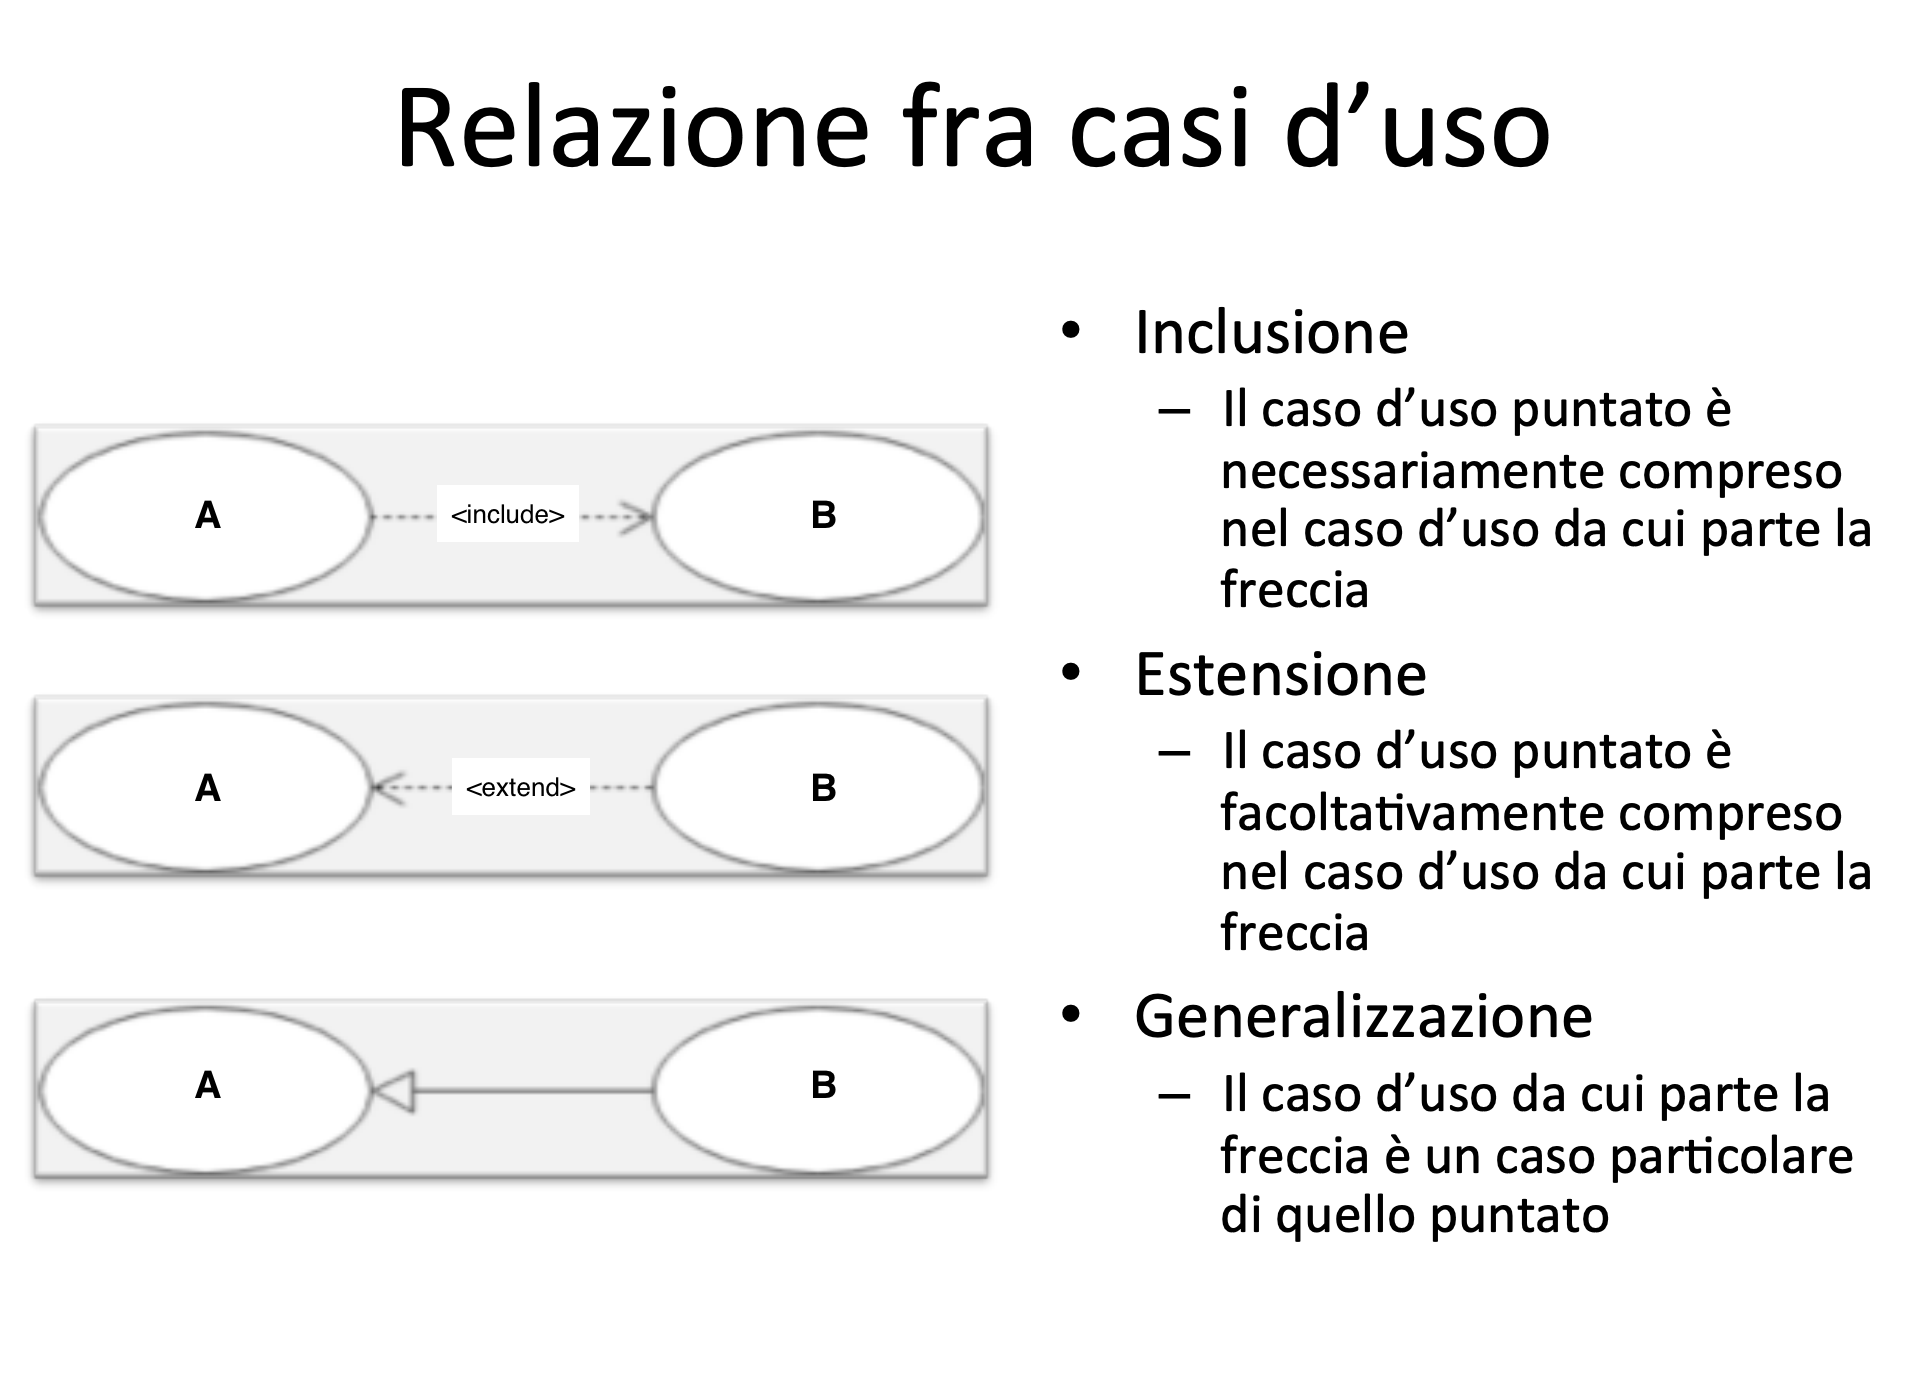
\includegraphics[width=0.8\textwidth]{immagini/uml_use_case_relazioni.png} % Immagine da Pagina 2 del tuo UML.pdf
    \caption{Rappresentazione grafica delle relazioni comuni tra Casi d'Uso in UML (Inclusione, Estensione e Generalizzazione).}
    \label{fig:uml_use_case_relazioni}
\end{figure}

\paragraph{Esempio Completo: Sistema di Ristorazione}
Un esempio pratico aiuta a consolidare la comprensione di come i casi d'uso e le loro relazioni si applichino in un contesto reale. Il diagramma seguente mostra le funzionalità di un sistema di gestione per un ristorante, illustrando le interazioni tra clienti, personale e il sistema stesso.
\begin{figure}[h!]
    \centering
    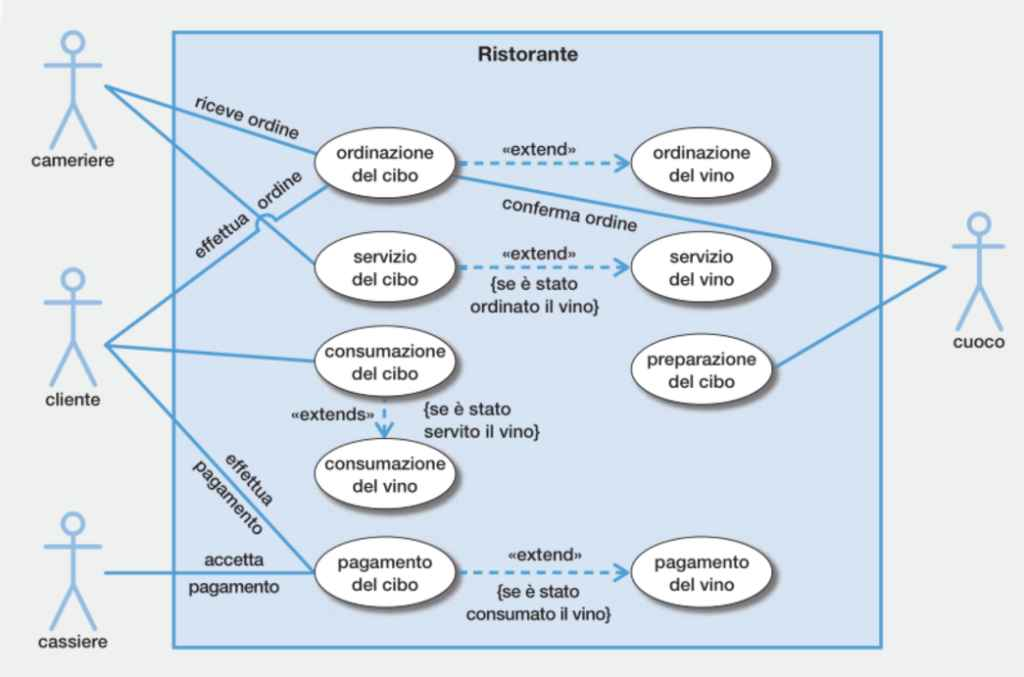
\includegraphics[width=0.9\textwidth]{immagini/diagramma_casi_uso_ristorante.jpg} % Immagine da Pagina 1 del tuo UML.pdf
    \caption{Esempio completo di Diagramma dei Casi d'Uso per un sistema di Ristorazione, che illustra le interazioni tra attori (Cameriere, Cliente, Cuoco, Cassiere) e le funzionalità del sistema.}
    \label{fig:diagramma_casi_uso_ristorante_completo}
\end{figure}

\subsubsection{Diagrammi delle Classi (Class Diagrams)}
I \textbf{Diagrammi delle Classi} sono diagrammi strutturali UML che mostrano la struttura statica di un sistema, le classi, i loro attributi (dati), i loro metodi (operazioni) e le relazioni tra le classi. Sono fondamentali per la progettazione orientata agli oggetti e per modellare il design logico del database.

\begin{itemize}
    \item \textbf{Scopo}: Modellare il design logico del sistema, la struttura del codice, le relazioni tra le classi e le dipendenze. Utile per visualizzare l'architettura del software a livello di classi.
    \item \textbf{Componenti Principali}:
    \begin{itemize}
        \item \textbf{Classe}: Rappresentata da un rettangolo diviso in tre sezioni: nome della classe, attributi (con visibilità e tipo), e metodi (con visibilità, parametri e tipo di ritorno).
        \item \textbf{Visibilità (Visibility)}: Indica l'accessibilità degli attributi e metodi, rappresentata da simboli specifici (\lstinline{+}, \lstinline{-}, \lstinline{\#}, \lstinline{\textasciitilde}).
        \item \textbf{Relazioni}: Specificano le associazioni tra le classi.
    \end{itemize}
\end{itemize}

\paragraph{Struttura Base e Attributi}
Un diagramma delle classi inizia con la rappresentazione della singola classe, evidenziando il suo nome, i suoi attributi (le proprietà) e le sue operazioni (i metodi).
\begin{figure}[h!]
    \centering
    \subcaptionbox{Struttura di una Classe (Automobile)\label{fig:class_base_automobile}}{%
        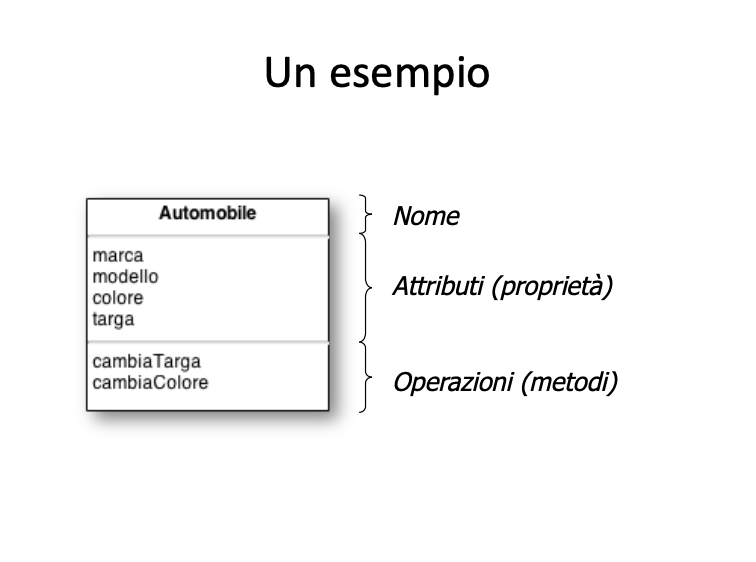
\includegraphics[width=0.45\textwidth]{immagini/uml_class_base_automobile.png}%
    }\quad
    \subcaptionbox{Classe con Metodi e Attributi (Scheda Anagrafica)\label{fig:class_scheda_anagrafica}}{%
        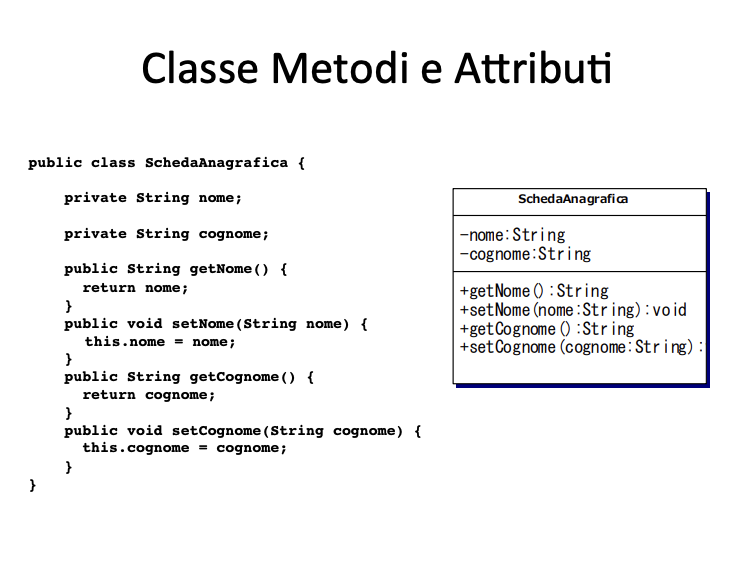
\includegraphics[width=0.45\textwidth]{immagini/uml_class_scheda_anagrafica_struttura.png}%
    }
    \caption{Esempi di rappresentazione base di una classe UML, con attributi e metodi, e come si relaziona al codice.}
    \label{fig:struttura_base_classi}
\end{figure}

L'uso di modificatori di visibilità definisce l'accessibilità di questi attributi e metodi, come mostrato nell'esempio dei Clienti e Fornitori.
\begin{figure}[h!]
    \centering
    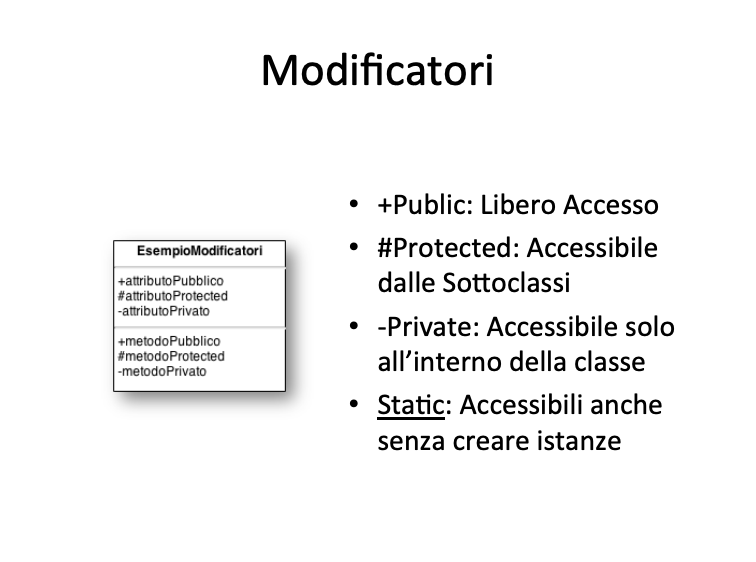
\includegraphics[width=0.7\textwidth]{immagini/uml_class_modificatori_visibilita.png}
    \caption{Esempio di Diagramma delle Classi che illustra l'uso dei modificatori di visibilità (public, private, protected) per attributi e metodi.}
    \label{fig:class_modificatori}
\end{figure}

\paragraph{Relazioni di Generalizzazione (Ereditarietà)}
La generalizzazione indica che una classe (sottoclasse) eredita proprietà e comportamenti da un'altra classe (superclasse). Questo promuove il riutilizzo del codice.
\begin{figure}[h!]
    \centering
    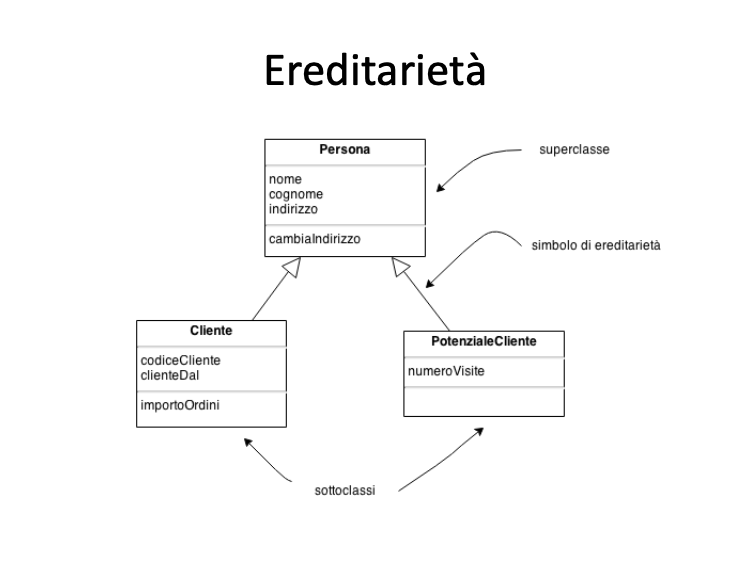
\includegraphics[width=0.7\textwidth]{immagini/uml_class_ereditarieta_generica.png}
    \caption{Esempio di Diagramma delle Classi che mostra la relazione di ereditarietà tra le classi Persona, Cliente e Potenziale Cliente.}
    \label{fig:class_ereditarieta}
\end{figure}
In contesti come Java, dove l'ereditarietà multipla non è ammessa (a differenza di C++), le interfacce vengono utilizzate per ovviare a questa limitazione, permettendo a una classe di implementare più interfacce.
\begin{figure}[h!]
    \centering
    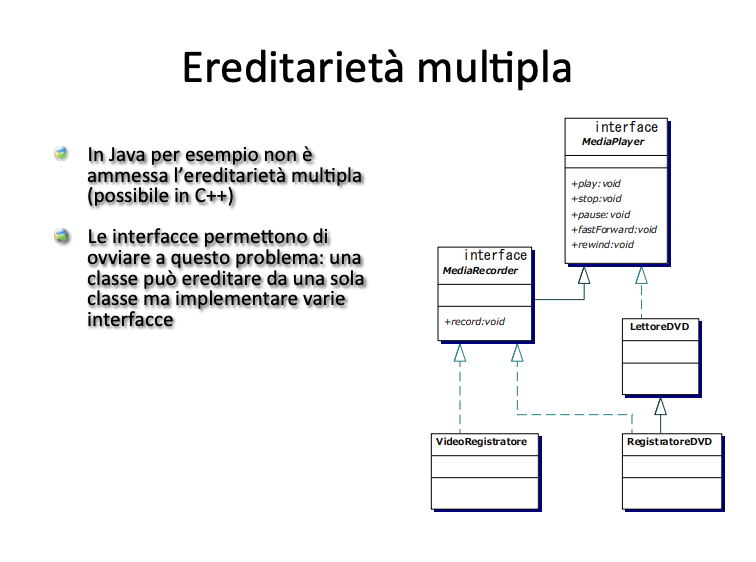
\includegraphics[width=0.7\textwidth]{immagini/uml_class_ereditarieta_multipla_interfacce.png}
    \caption{Esempio di Diagramma delle Classi che illustra come le interfacce consentono di simulare l'ereditarietà multipla in linguaggi che non la supportano nativamente.}
    \label{fig:class_ereditarieta_multipla}
\end{figure}

\paragraph{Relazioni Strutturali: Aggregazione e Composizione}
Aggregazione e composizione sono forme specifiche di associazione che esprimono relazioni "parte di" tra classi, distinguendosi per la dipendenza esistenziale della parte rispetto al tutto.
\begin{itemize}
    \item \textbf{Aggregazione}: Rappresenta una relazione uno a molti in cui l'oggetto "parte" può esistere indipendentemente dall'oggetto "tutto" (es. un libro può esistere senza una mensola specifica). Viene rappresentata con una freccia con la punta a diamante vuota all'estremità del "tutto".
    \item \textbf{Composizione}: Una forma più forte di aggregazione, che implica una esclusività. La "parte" non può esistere da sola senza il "tutto", e la distruzione del "tutto" comporta la distruzione delle "parti" (es. una pagina non può esistere senza il suo libro). Il diamante si disegna pieno.
\end{itemize}
\begin{figure}[h!]
    \centering
    \subcaptionbox{Esempio di Aggregazione (Mensola e Libro)\label{fig:class_aggregazione_esempio}}{%
        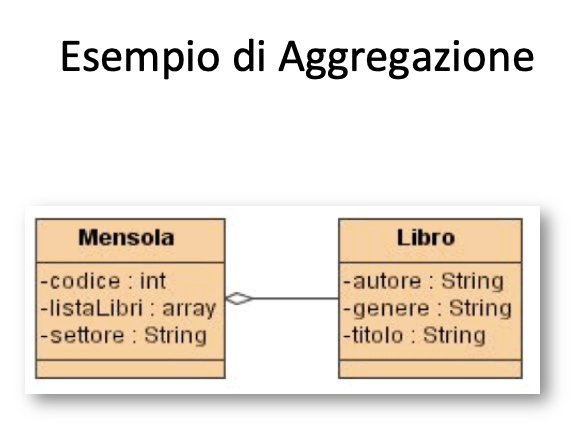
\includegraphics[width=0.45\textwidth]{immagini/uml_class_aggregazione_esempio.png}%
    }\quad
    \subcaptionbox{Esempio di Composizione (Libro e Pagina)\label{fig:class_composizione_esempio}}{%
        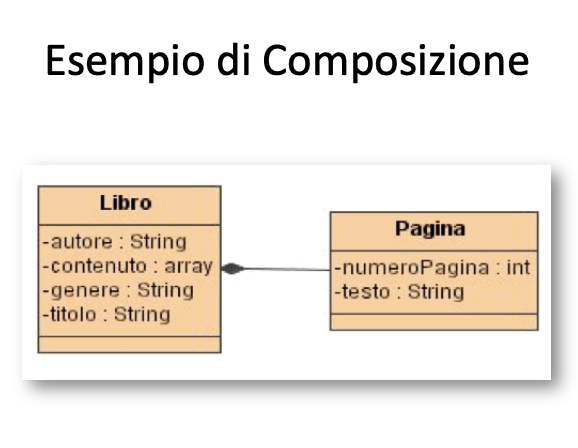
\includegraphics[width=0.45\textwidth]{immagini/uml_class_composizione_esempio.png}%
    }
    \caption{Confronto visivo tra Aggregazione e Composizione nei Diagrammi delle Classi UML.}
    \label{fig:class_aggregazione_composizione}
\end{figure}

\paragraph{Esempi Complessi di Diagrammi delle Classi}
Per illustrare l'applicazione di queste relazioni in contesti più ampi, consideriamo sistemi con diverse classi interconnesse, come un sistema e-commerce o un'applicazione di chat. Questi esempi mostrano come le classi interagiscono per formare un sistema coerente.
\begin{figure}[h!]
    \centering
    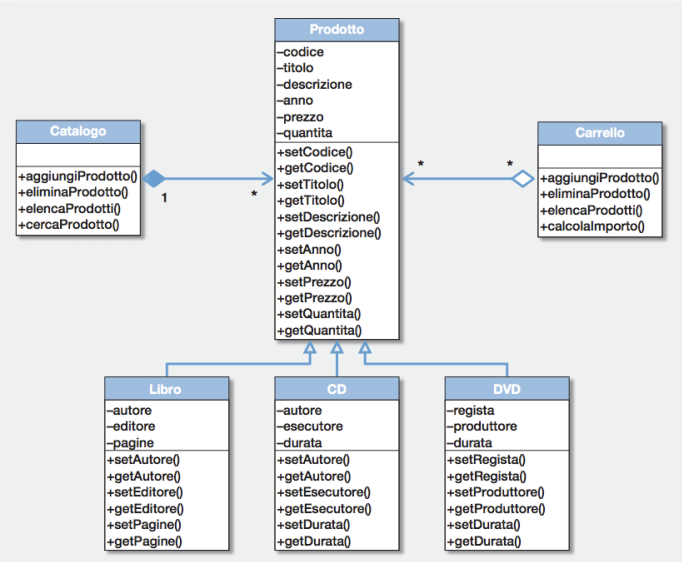
\includegraphics[width=0.9\textwidth]{immagini/uml_class_sistema_e_commerce.png} % Assicurati che l'immagine sia salvata con questo nome e percorso
    \caption{Diagramma delle Classi per un sistema di gestione prodotti/catalogo/carrello, che illustra varie classi e le loro relazioni (es. Prodotto, Carrello, DVD, Libro).}
    \label{fig:class_sistema_e_commerce}
\end{figure}
\begin{figure}[h!]
    \centering
    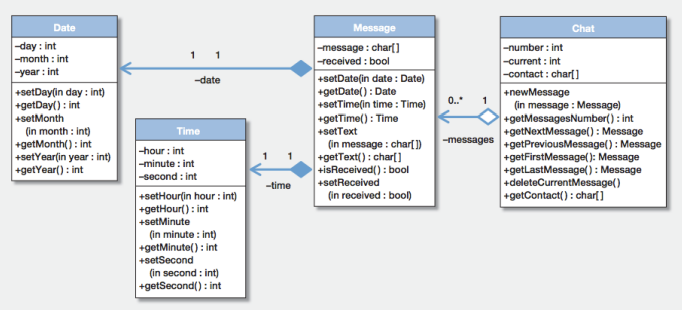
\includegraphics[width=0.9\textwidth]{immagini/uml_class_sistema_chat_corretto.png} % Assicurati che l'immagine sia salvata con questo nome e percorso
    \caption{Diagramma delle Classi per un sistema di Chat, che mostra le interazioni tra classi come Utente, Chat e Messaggio, e le loro molteplicità.}
    \label{fig:class_sistema_chat}
\end{figure}

\subsubsection{Diagrammi di Sequenza (Sequence Diagrams)}
I \textbf{Diagrammi di Sequenza} sono diagrammi comportamentali (di interazione) UML che mostrano l'ordine cronologico dei messaggi scambiati tra oggetti o attori in un'interazione specifica. Sono usati per modellare la logica di una funzionalità o di un algoritmo, illustrando come diversi oggetti collaborano per raggiungere un obiettivo.
\begin{itemize}
    \item \textbf{Scopo}: Dettagliare il flusso di controllo e di dati per funzionalità specifiche, spesso come implementazione di casi d'uso. Utili per visualizzare l'interazione dinamica e l'ordine delle chiamate.
    \item \textbf{Componenti Principali}:
    \begin{itemize}
        \item \textbf{Lifeline (Linea di Vita)}: Rappresenta la partecipazione di un oggetto o attore all'interazione, mostrata come una linea verticale tratteggiata. In cima alla lifeline c'è un rettangolo (per gli oggetti) o un omino (per gli attori).
        \item \textbf{Attore}: Utente o sistema esterno che avvia o partecipa all'interazione.
        \item \textbf{Messaggio}: Una comunicazione o chiamata di metodo tra lifeline, rappresentata da una freccia orizzontale. Possono essere:
        \begin{itemize}
            \item \textbf{Sincroni}: Freccia piena, indica una chiamata bloccante in attesa di risposta.
            \item \textbf{Asincroni}: Freccia con punta aperta, indica una chiamata non bloccante.
            \item \textbf{Risposta}: Freccia tratteggiata, indica il ritorno di un valore o la fine di una chiamata sincrona.
        \end{itemize}
        \item \textbf{Barra di Attivazione (Activation Bar/Execution Occurrence)}: Un rettangolo sottile posizionato verticalmente sulla lifeline, che indica il periodo di tempo durante il quale un oggetto è attivo e sta eseguendo un'operazione o aspettando una risposta.
        \item \textbf{Frammenti Combinati (Combined Fragments)}: Costrutti per mostrare strutture di controllo logico:
        \begin{itemize}
            \item \textbf{alt (alternative)}: Per mostrare blocchi if-else.
            \item \textbf{opt (optional)}: Per mostrare un blocco if.
            \item \textbf{loop (loop)}: Per mostrare iterazioni.
            \item \textbf{par (parallel)}: Per mostrare esecuzioni parallele.
        \end{itemize}
    \end{itemize}
\end{itemize}
\begin{figure}[h!]
    \centering
    % Placeholder per l'immagine del Diagramma di Sequenza UML
    % \includegraphics[width=0.8\textwidth]{immagini/diagramma_sequenza_esempio.png}
    \caption{Esempio di Diagramma di Sequenza UML che mostra l'interazione temporale degli oggetti per una funzionalità.}
    \label{fig:diagramma_sequenza_uml_specifico}
\end{figure}

\subsubsection{Diagrammi di Deployment (Deployment Diagrams)}
I \textbf{Diagrammi di Deployment} sono diagrammi strutturali UML che mostrano la configurazione fisica dei nodi hardware (computer, server, dispositivi) e come i componenti software sono distribuiti su questi nodi.
\begin{itemize}
    \item \textbf{Scopo}: Visualizzare la topologia fisica del sistema, la distribuzione dei componenti software sull'hardware e le interazioni fisiche tra i nodi. Utile per architetture distribuite e pianificazione dell'infrastruttura.
    \item \textbf{Componenti Principali}:
    \begin{itemize}
        \item \textbf{Nodo (Node)}: Una risorsa computazionale fisica o logica (hardware come un server, un PC, un dispositivo mobile; o un ambiente di esecuzione software come un Docker container, una JVM). Rappresentato da un cubo 3D.
        \item \textbf{Artefatto (Artifact)}: Un prodotto fisico risultante dal processo di sviluppo del software (file eseguibile, libreria, file JAR, file di configurazione, script). Rappresentato da un documento con l'icona di un artefatto.
        \item \textbf{Componente (Component)}: Una parte modulare e sostituibile del sistema con interfacce ben definite. Può essere distribuito su un nodo.
        \item \textbf{Comunicazione (Communication Path)}: Una linea che connette i nodi, indicando un percorso di comunicazione tra di essi (es. TCP/IP, HTTP).
    \end{itemize}
\end{itemize}
\begin{figure}[h!]
    \centering
    % Placeholder per l'immagine del Diagramma di Deployment UML
    % \includegraphics[width=0.8\textwidth]{immagini/diagramma_deployment_esempio.png}
    \caption{Esempio di Diagramma di Deployment UML che illustra la distribuzione dei componenti software sull'infrastruttura hardware.}
    \label{fig:diagramma_deployment_uml}
\end{figure}
\chapter{Elettronica}

L'\textbf{Elettronica} è la branca dell'ingegneria e della fisica che si occupa del controllo del flusso di elettroni, tipicamente attraverso dispositivi semiconduttori, per costruire circuiti e sistemi che elaborano informazioni o controllano energia. È alla base di tutti i dispositivi digitali e di molteplici sistemi analogici moderni.

\section{Transistore MOS (Metal-Oxide-Semiconductor Field-Effect Transistor)}
Il \textbf{transistore MOS} è il dispositivo fondamentale della microelettronica moderna e la spina dorsale di microprocessori, memorie e altri circuiti integrati. È un transistore a effetto di campo (FET), dove la corrente tra due terminali (Source e Drain) è controllata da un campo elettrico generato da una tensione applicata a un terzo terminale (Gate).

\subsection{Struttura del Transistore MOS (nMOS)}
Per comprendere il funzionamento, si consideri la realizzazione più comune: l'nMOS (n-channel Metal-Oxide-Semiconductor).
\begin{itemize}
    \item \textbf{Substrato (Bulk/Body)}: Generalmente di tipo P per un nMOS. È il materiale semiconduttore di base su cui viene costruito il dispositivo.
    \item \textbf{Source (S) e Drain (D)}: Due regioni altamente drogate (N+ per nMOS) impiantate nel substrato P. Sono simmetriche e collegate ai terminali esterni. Il Source è tipicamente la sorgente di portatori di carica, il Drain è dove fluiscono.
    \item \textbf{Canale}: La regione del substrato (P) tra Source e Drain. È qui che si formerà il canale di conduzione per il flusso di corrente.
    \item \textbf{Ossido di Gate ($SiO_2$)}: Uno strato isolante molto sottile (diossido di silicio) deposto sopra il canale. Agisce come dielettrico, isolando elettricamente il Gate dal canale.
    \item \textbf{Gate (G)}: Uno strato conduttivo (metallo o polisilicio) deposto sopra l'ossido di gate. È il terminale di controllo attraverso il quale si applica la tensione per creare il campo elettrico.
    \item \textbf{Terminali}: Gate (G), Source (S), Drain (D), Bulk/Substrate (B). Spesso il Bulk è collegato al Source o a una tensione fissa (es. massa per nMOS, $V_{DD}$ per pMOS).
\end{itemize}

\subsection{Principio di Funzionamento (nMOS)}
Il funzionamento del transistore MOS dipende dalla tensione applicata tra Gate e Source ($V_{GS}$) e tra Drain e Source ($V_{DS}$). Si basa sulla modulazione della conduttività del canale tramite un campo elettrico.
\begin{itemize}
    \item \textbf{Interdizione (Cut-off Region)}:
    \begin{itemize}
        \item \textbf{Condizione}: $V_{GS} < V_{TH}$ (Tensione di Soglia).
        \item \textbf{Descrizione}: Non c'è un campo elettrico sufficiente per attrarre elettroni al canale. Non si forma un canale di conduzione tra Source e Drain. La corrente $I_{DS}$ è praticamente nulla (solo una piccola corrente di leakage). Il transistore agisce come un interruttore aperto.
    \end{itemize}
    \item \textbf{Conduzione (quando $V_{GS} > V_{TH}$)}:
    \begin{itemize}
        \item Quando una tensione positiva $V_{GS}$ sufficiente (maggiore di $V_{TH}$) viene applicata al Gate, il campo elettrico attrae gli elettroni (portatori minoritari nel substrato P) verso la superficie del semiconduttore, sotto l'ossido.
        \item Si forma uno strato sottile di elettroni, creando un \textbf{canale di conduzione} a bassa resistenza tra Source e Drain.
        \item Se si applica una tensione $V_{DS} > 0$, una corrente $I_{DS}$ fluirà attraverso questo canale.
    \end{itemize}
\end{itemize}

\subsection{Regimi di Funzionamento (per nMOS con $V_{GS} > V_{TH}$)}
Una volta che il transistore è in conduzione, il suo comportamento (e la corrente $I_{DS}$) dipende dalla relazione tra $V_{GS}$ e $V_{DS}$.
\begin{itemize}
    \item \textbf{Regione di Triodo (o Lineare/Ohmica)}:
    \begin{itemize}
        \item \textbf{Condizioni}: $V_{GS} > V_{TH}$ e $V_{DS} < (V_{GS} - V_{TH})$.
        \item \textbf{Descrizione}: Il canale è completamente formato e la sua profondità è relativamente uniforme. Il transistore si comporta come una resistenza controllata in tensione, e la corrente $I_{DS}$ è approssimativamente lineare rispetto a $V_{DS}$.
    \item \textbf{Applicazione}: Usata come interruttore chiuso (ON) in circuiti digitali (con bassa resistenza) o come resistenza variabile in circuiti analogici.
    \end{itemize}
    \item \textbf{Regione di Saturazione}:
    \begin{itemize}
        \item \textbf{Condizioni}: $V_{GS} > V_{TH}$ e $V_{DS} \geq (V_{GS} - V_{TH})$.
        \item \textbf{Descrizione}: Aumentando $V_{DS}$, la tensione canale-gate verso il lato del Drain si riduce. Quando $V_{DS}$ raggiunge $V_{GS} - V_{TH}$, il canale si "pizzica" (pinch-off) vicino al Drain. Oltre questo punto, ulteriori aumenti di $V_{DS}$ non aumentano significativamente la corrente $I_{DS}$, che diventa quasi costante.
    \item \textbf{Applicazione}: Questa è la regione di funzionamento preferita per gli amplificatori (circuiti analogici) in quanto si comporta come una sorgente di corrente controllata in tensione, e per gli stati ON (logico '1') in circuiti digitali per un'elevata impedenza di uscita.
    \end{itemize}
\end{itemize}

\subsection{Vantaggi del MOS rispetto al Transistore Bipolare (BJT)}
Il transistore MOS ha soppiantato in gran parte il BJT nella microelettronica digitale e in molte applicazioni analogiche grazie a diversi vantaggi chiave:
\begin{itemize}
    \item \textbf{Alta Impedenza di Ingresso}: Il gate del MOS è isolato dall'ossido, il che lo rende quasi idealmente un circuito aperto con una corrente di gate praticamente nulla ($I_G \approx 0$). Questo riduce il carico sui circuiti precedenti e semplifica il design degli stadi di ingresso. Il BJT, invece, è controllato in corrente (corrente di base) e presenta un'impedenza di ingresso inferiore.
    \item \textbf{Minore Dissipazione di Potenza Statica (in CMOS)}: Nelle configurazioni Complementary MOS (CMOS), quando il circuito è in stato stabile (non commuta), uno dei transistori è sempre spento, eliminando un percorso di corrente diretto tra alimentazione e massa. Questo porta a una dissipazione di potenza statica estremamente bassa, fondamentale per dispositivi a batteria e circuiti ad alta integrazione. I BJT, anche quando "spenti", possono avere correnti di leakage maggiori e configurazioni logiche basate su BJT tendono a dissipare più potenza.
    \item \textbf{Scalabilità e Densità di Integrazione}: I MOS possono essere miniaturizzati molto più facilmente rispetto ai BJT, permettendo la realizzazione di circuiti integrati con miliardi di transistori su un singolo chip. La loro struttura planare si presta bene alla fabbricazione su larga scala.
    \item \textbf{Costo di Fabbricazione}: Il processo di fabbricazione MOS è generalmente più semplice e meno costoso rispetto a quello BJT, che richiede più passaggi di drogaggio e diffusione.
    \item \textbf{Immunità al Rumore (in CMOS)}: I circuiti CMOS hanno buoni margini di rumore, rendendoli robusti contro le fluttuazioni di tensione indesiderate.
\end{itemize}
Nonostante ciò, i BJT mantengono vantaggi in alcune applicazioni specifiche (es. alta frequenza, alta potenza) grazie a una maggiore transconduttanza e velocità in particolari contesti.

\section{Circuiti CMOS (Complementary MOS)}
La tecnologia \textbf{CMOS} è il design più diffuso per la realizzazione di circuiti integrati digitali, caratterizzata dall'uso complementare di transistori nMOS e pMOS.

\subsection{Invertitore CMOS}
L'\textbf{invertitore CMOS} è la porta logica fondamentale in tecnologia CMOS, che realizza la funzione NOT (negazione logica). Produce un'uscita opposta all'ingresso.
\begin{itemize}
    \item \textbf{Realizzazione}: È composto da due transistori MOS collegati in serie tra $V_{DD}$ e GND, con i gate collegati insieme a formare l'ingresso (IN) e i drain collegati a formare l'uscita (OUT).
    \begin{itemize}
        \item Un \textbf{pMOS} (pull-up network) è collegato tra $V_{DD}$ e OUT. Il pMOS conduce quando il suo gate è basso.
        \item Un \textbf{nMOS} (pull-down network) è collegato tra OUT e GND. L'nMOS conduce quando il suo gate è alto.
    \end{itemize}
    \item \textbf{Funzionamento}:
    \begin{itemize}
        \item \textbf{Ingresso Alto (Logico '1', $V_{IN} = V_{DD}$)}: L'nMOS è ON (conduce), creando un percorso a bassa resistenza tra OUT e GND. Il pMOS è OFF (interdetto). L'uscita $V_{OUT}$ è tirata a GND (Logico '0').
        \item \textbf{Ingresso Basso (Logico '0', $V_{IN} = GND$)}: Il pMOS è ON (conduce), creando un percorso a bassa resistenza tra OUT e $V_{DD}$. L'nMOS è OFF (interdetto). L'uscita $V_{OUT}$ è tirata a $V_{DD}$ (Logico '1').
    \end{itemize}
\end{itemize}

\subsection{Vantaggi dell'Invertitore CMOS rispetto agli Invertitori con Carico Resistivo}
Gli invertitori CMOS offrono vantaggi significativi rispetto alle implementazioni più vecchie che usavano un transistore (BJT o MOS) con una resistenza di carico:
\begin{itemize}
    \item \textbf{Minore Dissipazione di Potenza Statica (Vantaggio Primario)}: Nello stato stabile (ingresso alto o basso), uno dei due transistori (nMOS o pMOS) è sempre spento. Non c'è un percorso di corrente diretto da $V_{DD}$ a GND. La corrente statica è limitata a correnti di leakage quasi nulle, risultando in un consumo di potenza estremamente basso a riposo. Gli invertitori con carico resistivo, invece, dissipano continuamente potenza quando l'uscita è nello stato "basso", poiché la corrente fluisce attraverso il resistore di carico e il transistore acceso.
    \item \textbf{Migliori Margini di Rumore}: Le curve di trasferimento tensione-tensione degli invertitori CMOS sono quasi ideali, con una transizione molto ripida tra i due stati logici. Questo fornisce ampi margini di rumore, rendendo i circuiti più robusti alle fluttuazioni di tensione indesiderate.
    \item \textbf{Prestazioni Simmetriche (Potenziale)}: Con un corretto dimensionamento dei transistori (rapporto $W/L$), i tempi di salita (charge time) e di discesa (discharge time) dell'uscita possono essere resi quasi simmetrici. Negli invertitori con resistore, il tempo di salita (carica del condensatore di carico attraverso il resistore) è tipicamente più lento del tempo di discesa.
    \item \textbf{Densità di Integrazione}: I transistori MOS occupano meno area rispetto ai resistori su chip, consentendo una maggiore densità di circuiti.
\item \textbf{Ampio Range di Tensione Operativa}: I circuiti CMOS possono operare su un'ampia gamma di tensioni di alimentazione mantenendo buone prestazioni.
\end{itemize}

\subsection{Applicazioni Notevoli dell'Invertitore CMOS}
L'invertitore CMOS è un blocco costruttivo fondamentale per una vasta gamma di applicazioni:
\begin{itemize}
    \item \textbf{Porta Logica Fondamentale}: È il componente di base da cui vengono costruite tutte le altre porte logiche digitali (NAND, NOR, XOR, latch, flip-flop) in tecnologia CMOS.
    \item \textbf{Buffer e Driver}: Utilizzando cascate di invertitori, si possono creare buffer (per aumentare la capacità di pilotaggio di un segnale) o driver per linee lunghe o carichi capacitivi elevati (es. clock network nei microprocessori).
    \item \textbf{Celle di Memoria}: Due invertitori CMOS collegati in back-to-back formano un latch, che è la cella di memoria fondamentale nelle SRAM (Static RAM), capace di memorizzare un bit.
    \item \textbf{Oscillatori ad Anello (Ring Oscillators)}: Una catena di un numero dispari di invertitori, con l'uscita dell'ultimo collegata all'ingresso del primo, crea un oscillatore che produce un'onda quadra. Usati per testare le prestazioni di velocità e per generare segnali di clock.
    \item \textbf{Livelli di Tensione}: Possono essere usati per convertire livelli di tensione logici tra diversi standard o blocchi di circuiti.
\end{itemize}

\chapter{Sistemi Numerici}

I \textbf{sistemi numerici} sono metodi per rappresentare i numeri utilizzando simboli specifici e regole ben definite. In informatica, la rappresentazione binaria è fondamentale, ma è cruciale anche capire come i numeri negativi vengono gestiti, in particolare tramite il complemento a due.

\section{Rappresentazione per Numeri Interi}
I numeri interi possono essere rappresentati in diversi modi all'interno di un sistema digitale. Le rappresentazioni più comuni per i numeri con segno includono segno e modulo, complemento a uno, e complemento a due. Il complemento a due è la rappresentazione più utilizzata nei sistemi digitali moderni per la sua efficienza nelle operazioni aritmetiche.

\subsection{Complemento a Due}
La rappresentazione in \textbf{complemento a due} è il metodo più diffuso per rappresentare numeri interi con segno nei sistemi digitali. Offre il vantaggio di semplificare le operazioni di somma e sottrazione, poiché la sottrazione può essere implementata come una somma con il complemento a due del sottraendo, eliminando la necessità di circuiti dedicati alla sottrazione.

\subsubsection{Principio di Funzionamento}
\begin{itemize}
    \item Un numero positivo in complemento a due è rappresentato esattamente come nella notazione binaria pura (senza segno), con il bit più significativo (MSB) pari a 0.
    \item Un numero negativo in complemento a due è ottenuto complementando (invertendo) tutti i bit del suo valore assoluto (passando dal 0 all'1 e viceversa) e poi sommando 1 al risultato. Il bit più significativo (MSB) sarà sempre 1 per i numeri negativi.
    \item Il bit più significativo (MSB) indica il segno: 0 per i positivi, 1 per i negativi.
    \item Il range di valori rappresentabile con $N$ bit in complemento a due va da $-2^{N-1}$ a $2^{N-1}-1$. Ad esempio, con 8 bit, si possono rappresentare numeri da $-128$ a $127$.
\end{itemize}

\subsubsection{Derivazione della Rappresentazione in Complemento a Due}
Per convertire un numero decimale negativo in complemento a due (con $N$ bit):
\begin{enumerate}
    \item Prendi il valore assoluto del numero decimale (positivo).
    \item Converti il valore assoluto in binario su $N$ bit.
    \item Inverti tutti i bit (complemento a uno, 0 diventa 1, 1 diventa 0).
    \item Somma 1 al risultato binario.
\end{enumerate}
Per convertire un numero binario in complemento a due a decimale:
\begin{itemize}
    \item Se il MSB è 0: il numero è positivo. Convertilo come un normale binario senza segno.
    \item Se il MSB è 1: il numero è negativo.
    \begin{enumerate}
        \item Inverti tutti i bit del numero binario.
        \item Somma 1 al risultato binario.
        \item Converti questo risultato binario in decimale e anteponi il segno meno.
    \end{enumerate}
\end{itemize}

\subsubsection{Esempio: Rappresentazione in Binario a 16 bit del numero decimale -15}
Per rappresentare il numero decimale -15 in complemento a due su 16 bit:
\begin{enumerate}
    \item \textbf{Valore assoluto}: $|-15| = 15$.
    \item \textbf{15 in binario su 16 bit}: $0000\,0000\,0000\,1111_2$.
    \item \textbf{Inverti tutti i bit (complemento a uno)}: $1111\,1111\,1111\,0000_2$.
    \item \textbf{Somma 1}: $1111\,1111\,1111\,0000_2 + 1_2 = 1111\,1111\,1111\,0001_2$.
\end{enumerate}
Quindi, la rappresentazione in complemento a due di -15 su 16 bit è $1111\,1111\,1111\,0001_2$.

\section{Operazioni Aritmetiche con Complemento a Due}
Il vantaggio principale del complemento a due è che le operazioni di addizione e sottrazione possono essere eseguite utilizzando lo stesso circuito per l'addizione.

\subsection{Addizione}
L'addizione di due numeri (positivi o negativi) in complemento a due viene eseguita come una normale addizione binaria. Qualsiasi bit di riporto che esce dal bit più significativo (MSB) viene semplicemente ignorato.
\begin{itemize}
    \item \textbf{Esempio}: $5 + (-2)$ su 4 bit ($N=4$, range da -8 a 7)
    \begin{itemize}
        \item $5_{10} = 0101_2$
        \item $-2_{10}$:
        \begin{itemize}
            \item $2_{10} = 0010_2$
            \item Complemento a uno: $1101_2$
            \item Somma 1: $1101_2 + 1_2 = 1110_2$ (che è $-2_{10}$ in complemento a due)
        \end{itemize}
        \item \textbf{Somma}:
        \begin{lstlisting}[language=Pseudocode]
  0101  (5)
+ 1110  (-2)
-----
 10011
        \end{lstlisting}
        Il bit di riporto (il primo 1 a sinistra) viene ignorato. Il risultato è $0011_2 = 3_{10}$, che è corretto.
    \end{itemize}
\end{itemize}

\subsection{Sottrazione}
La sottrazione $A - B$ è implementata come la somma $A + (-B)$. Per calcolare $-B$, si determina il complemento a due di $B$.
\begin{itemize}
    \item \textbf{Esempio}: $5 - 2$ su 4 bit ($N=4$, range da -8 a 7)
    \begin{itemize}
        \item $5_{10} = 0101_2$
        \item $-2_{10} = 1110_2$ (già calcolato sopra)
        \item \textbf{Sottrazione come somma}: $5 + (-2)$
        \begin{lstlisting}[language=Pseudocode]
  0101  (5)
+ 1110  (-2)
-----
 10011
        \end{lstlisting}
        Ignorando il riporto, il risultato è $0011_2 = 3_{10}$, che è corretto.
    \end{itemize}
\end{itemize}

\subsection{Overflow}
L'\textbf{overflow} si verifica quando il risultato di un'operazione aritmetica supera il range di valori rappresentabili con il numero di bit a disposizione.
\begin{itemize}
    \item \textbf{Rilevamento}: Si verifica un overflow se:
    \begin{itemize}
        \item Si sommano due numeri positivi e il risultato è negativo.
        \item Si sommano due numeri negativi e il risultato è positivo.
        \item Un modo più formale per rilevarlo è controllare se il riporto nel bit del segno (MSB) è diverso dal riporto fuori dal bit del segno.
    \end{itemize}
\end{itemize}

% --- Se vuoi aggiungere appendici per soluzioni dettagliate di esercizi o altro ---
% \appendix
% \chapter{Soluzioni Dettagliate e Approfondimenti}
% \include{capitoli/basi_di_dati/esercizi/es_er_campi} % Esempio: inclusione di un file di esercizio

\backmatter % Sezione finale del libro (ad es. bibliografia, indici analitici)

\printbibliography % Stampa la bibliografia. Questo comando è fornito da biblatex.

\end{document}